\chapter{Systematic Uncertainties}
\label{chap:syst}

The systematic uncertainties in the signal efficiency is estimated by estimating the systematic uncertainty of each efficiency factor in Eq.~\ref{eq:OverallEff} when possible. 

The systematic uncertainty in track and vertex reconstruction is studied using $K_{S}$ in Section~\ref{sec:syst:vertexing}. The systematic uncertainty in trigger is studied in Section~\ref{sec:syst:trigger} using tag-and-probe method with $Z\rightarrow \ee,\mumu$ events. The systematic uncertainty in lepton reconstruction and identification cannot be estimated using data since no known particle exists in nature that has a long lifetime and mass larger than 10 GeV.















\section{Systematic Uncertainty in Track and Vertex Reconstruction}
\label{sec:syst:vertexing}

In a typical analysis, the systematic uncertainty in track and vertex reconstruction is estimated by the Inner Tracking Combined Performance group using the standard tracking setup. This result cannot be directly used for this analysis due to the special reconstruction setup described in Chapter~\ref{chap:reco}. Instead, the systematic uncertainty in track and vertex reconstruction is estimated by comparing vertex yields between the data and the MC samples using the process, $K_{S}\rightarrow\pi^{+}\pi^{-}$. This process is ideal for comparing the efficiencies in the data and the MC samples due to the long lifetime ($c\tau \sim26.8~\si{\mm}$) of $K_{S}$ and the decay mode that leaves two charged tracks. However, there are intrinsic differences between $K_{S}$ and signal long-lived particles such as mass and $p_{T}$. In order to understand the validity and the limitation of this method, the kinematic distributions of $K_{S}$ and $Z'$ found in this method are compared in Appendix~\ref{app:syst_Ks_Zp}.

Tracks originating from a $K_{S}$ decay can be reconstructed by either the standard tracking (ST) or the LRT algorithm, resulting in three categories of $K_{S}$ vertices: vertices with two \textit{standard tracks}, one standard track and one \textit{large-radius track}, and two large-radius tracks. $K_{S}$ Vertex yields in each category can be expressed by total $K_{S}$ produced in a sample and tracking and vertexing efficiency,

\begin{align}
    N_{\mathrm{ST}}  &= K_{S}~\mathrm{produced} \times (\epsilon_{\mathrm{ST}})^{2} \cdot \epsilon_{\mathrm{vertexing~on~ST}}, \nonumber \\
    N_{\mathrm{ST+LRT}}  &= K_{S}~\mathrm{produced} \times (\epsilon_{\mathrm{ST}} \cdot \epsilon_{\mathrm{LRT}}) \cdot \epsilon_{\mathrm{vertexing~on~ST}}, \nonumber \\
    N_{\mathrm{LRT}}&= K_{S}~\mathrm{produced} \times (\epsilon_{\mathrm{LRT}})^{2} \cdot \epsilon_{\mathrm{vertexing~on~LRT}},
\label{eq:Ks_eq1}
\end{align}

where $N$ represents vertex yields in each category. $\epsilon_{\mathrm{ST}}$ and $\epsilon_{\mathrm{LRT}}$ represent track reconstruction efficiency in the ST and the LRT, respectively. $\epsilon_{\mathrm{vertexing~on~ST}}$ or $\epsilon_{\mathrm{vertexing~on~LRT}}$ represents two-track vertex reconstruction efficiency on two standard or large-radius tracks, respectively.

In order to compare the efficiency in data and MC samples, the double ratio of data to MC is taken,
\begin{equation}
\dfrac{N_{\mathrm{LRT}} / N_{\mathrm{ST}}}{N_{\mathrm{LRT}}^{\mathrm{MC}} / N_{\mathrm{ST}}^{\mathrm{MC}}},
\label{eq:Ks_eq2}
\end{equation}

where quantities estimated using MC samples are denoted by MC, and quantities estimated using data are denoted otherwise. Using Eq.~\ref{eq:Ks_eq1} and the double ratio, the systematic uncertainty in track and vertex reconstruction is expressed as,

%\begin{align}
%    \dfrac{\dfrac{N_{LRT}}{N_{ST}}}{\dfrac{N'_{LRT}}{N'_{ST}}}  &= 
%        \dfrac
%        {\dfrac{(\epsilon_{\mathrm{LRT}})^{2} \cdot \epsilon_{\mathrm{vertexing~on~LRT}}}{(\epsilon_{\mathrm{ST}})^{2} \cdot \epsilon_{\mathrm{vertexing~on~ST}}}}
%        {\dfrac{(\epsilon'_{\mathrm{LRT}})^{2} \cdot \epsilon'_{\mathrm{vertexing~on~LRT}}}{(\epsilon'_{\mathrm{ST}})^{2} \cdot \epsilon'_{\mathrm{vertexing~on~ST}}}}
%\label{eq:Ks_eq2}
%\end{align}

\begin{align}
    \Big( \dfrac{\epsilon_{\mathrm{LRT}}}{\epsilon_{\mathrm{LRT}}^{\mathrm{MC}}}\Big)^{2} \cdot
    \Big( \dfrac{\epsilon_{\mathrm{vertexing~on~LRT}}}{\epsilon_{\mathrm{vertexing~on~LRT}}^{\mathrm{MC}}}\Big) &=
    \Big( \dfrac{N_{\mathrm{LRT}} \cdot N_{\mathrm{ST}}^{\mathrm{MC}}}{N_{\mathrm{LRT}}^{\mathrm{MC}} \cdot N_{\mathrm{ST}}} \Big) \cdot
    \Big( \dfrac{\epsilon_{\mathrm{ST}}}{\epsilon_{\mathrm{ST}}^{\mathrm{MC}}}\Big)^{2} \cdot
    \Big( \dfrac{\epsilon_{\mathrm{vertexing~on~ST}}}{\epsilon_{\mathrm{vertexing~on~ST}}^{\mathrm{MC}}}\Big).
\label{eq:Ks_eq3}
\end{align}

Together with the results from the ST studies, $K_{S}$ vertex yields from the data and the MC samples estimated in this study are used to estimate the difference in the LRT track and vertex reconstruction efficiency between the data and the MC samples.

Events are selected using the same event selection described in Section~\ref{sec:selection:pre} except trigger filters as the high-$p_{T}$ photon or muon triggers are not suitable for $K_{S}$ study. From the selected events, $K_{S}$ candidates, referred as $K_{S}$ vertices, are selected by applying $K_{S}$ vertex selection to secondary vertices in the events. The $K_{S}$ vertex selection is similar to the $Z'$ signal vertex selection, but for consistency with $K_{S}$ study in Run I and background reduction, additional vertex cuts described in Ref.~\cite{Aad:2011hd} are applied. The mass window of 0.35 to 0.65 GeV is used in the $K_{S}$ vertex selection. The difference between $K_{S}$ and $Z'$ vertex selections are summarized in Table~\ref{table:ks_vertex_cut}. Figure~\ref{fig:Ks_vertex_cutflow} shows $K_{S}$ vertex cut flow in the data and the background MC samples.

\begin{table}[!htb]
%\begin{table}[tb]
  \centering
  \begin{tabular}{ c c c }
    \hline
    \hline
                    & $Z'$                                                  & $K_{S}$                               \\
    \hline
    Trigger         & Photon or muon trigger (Table~\ref{table:triggers})    & -                                     \\
    Vertex type     & \mumu, \emu, \ee                                      & \xx                                   \\
    Mass (GeV)      & $> 10.0$                                              & $[0.35,0.65]$                         \\
    Additional cut  & -                                                     & $K_{S}$ selection~\cite{Aad:2011hd}   \\
    \hline
    \hline
  \end{tabular}
  \caption{Comparison of $Z'$ and $K_{S}$ vertex selections.}
  \label{table:ks_vertex_cut}
\end{table}

\begin{figure}[!htb]
	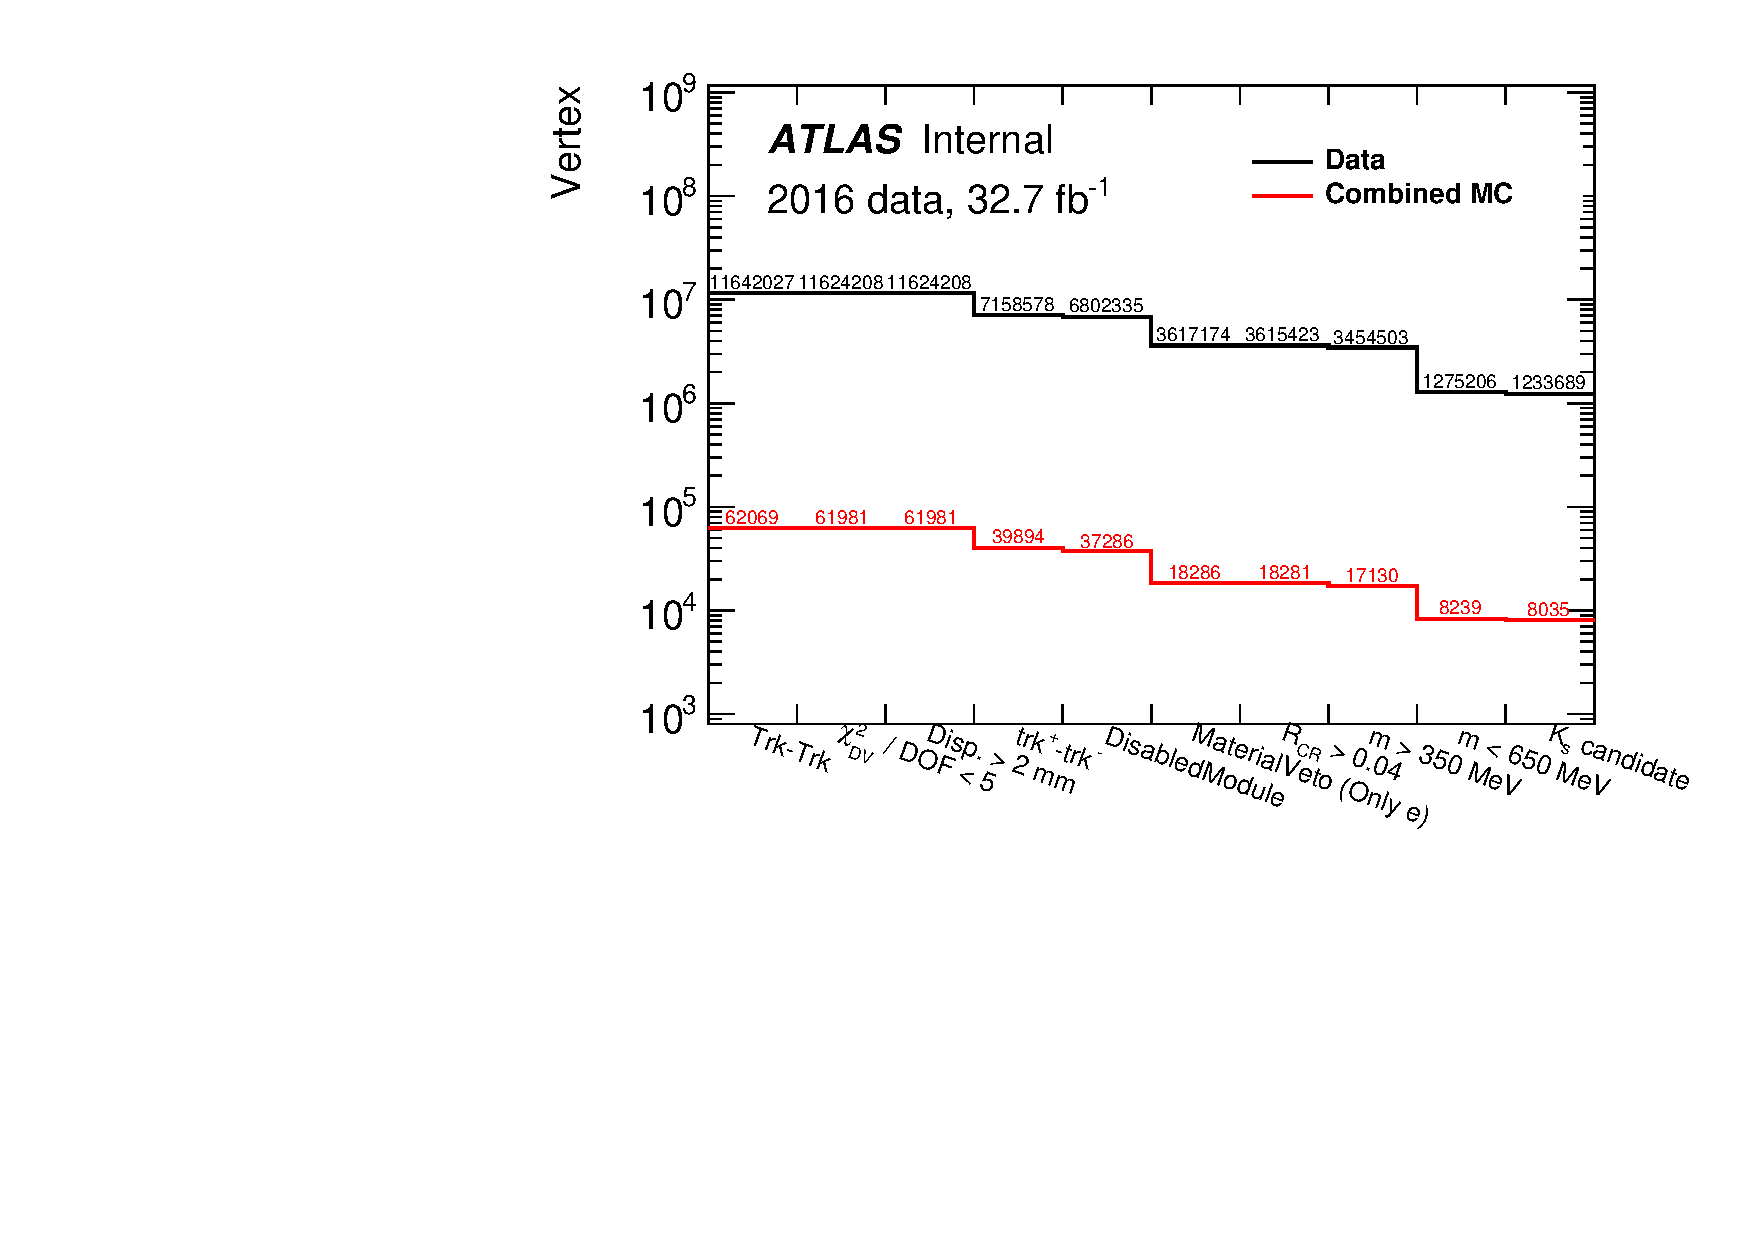
\includegraphics[width=0.60\textwidth]{figures/m_syst_Ks_cf.pdf}
	\centering
	\caption{Vertex cut flow applied on $K_{S}$ vertices in the data and the MC samples}
	\label{fig:Ks_vertex_cutflow}
\end{figure}

After applying the event and $K_{S}$ vertex selection, the $K_{S}$ vertex distributions are compared between the data and the MC samples in Figure~\ref{fig:Ks_data_MC}. The data sample is normalized to the MC samples which have limited statistics. Only $K_{S}$ vertices with two large-radius tracks are shown. The distributions show good agreement in the invariant mass, $p_{T}$, transverse, longitudinal position, and decay length of the vertices, except the pile-up distribution as expected.


\begin{figure}[!htb]
    \centering
    \subfloat[]{\label{subfig:Ks_m}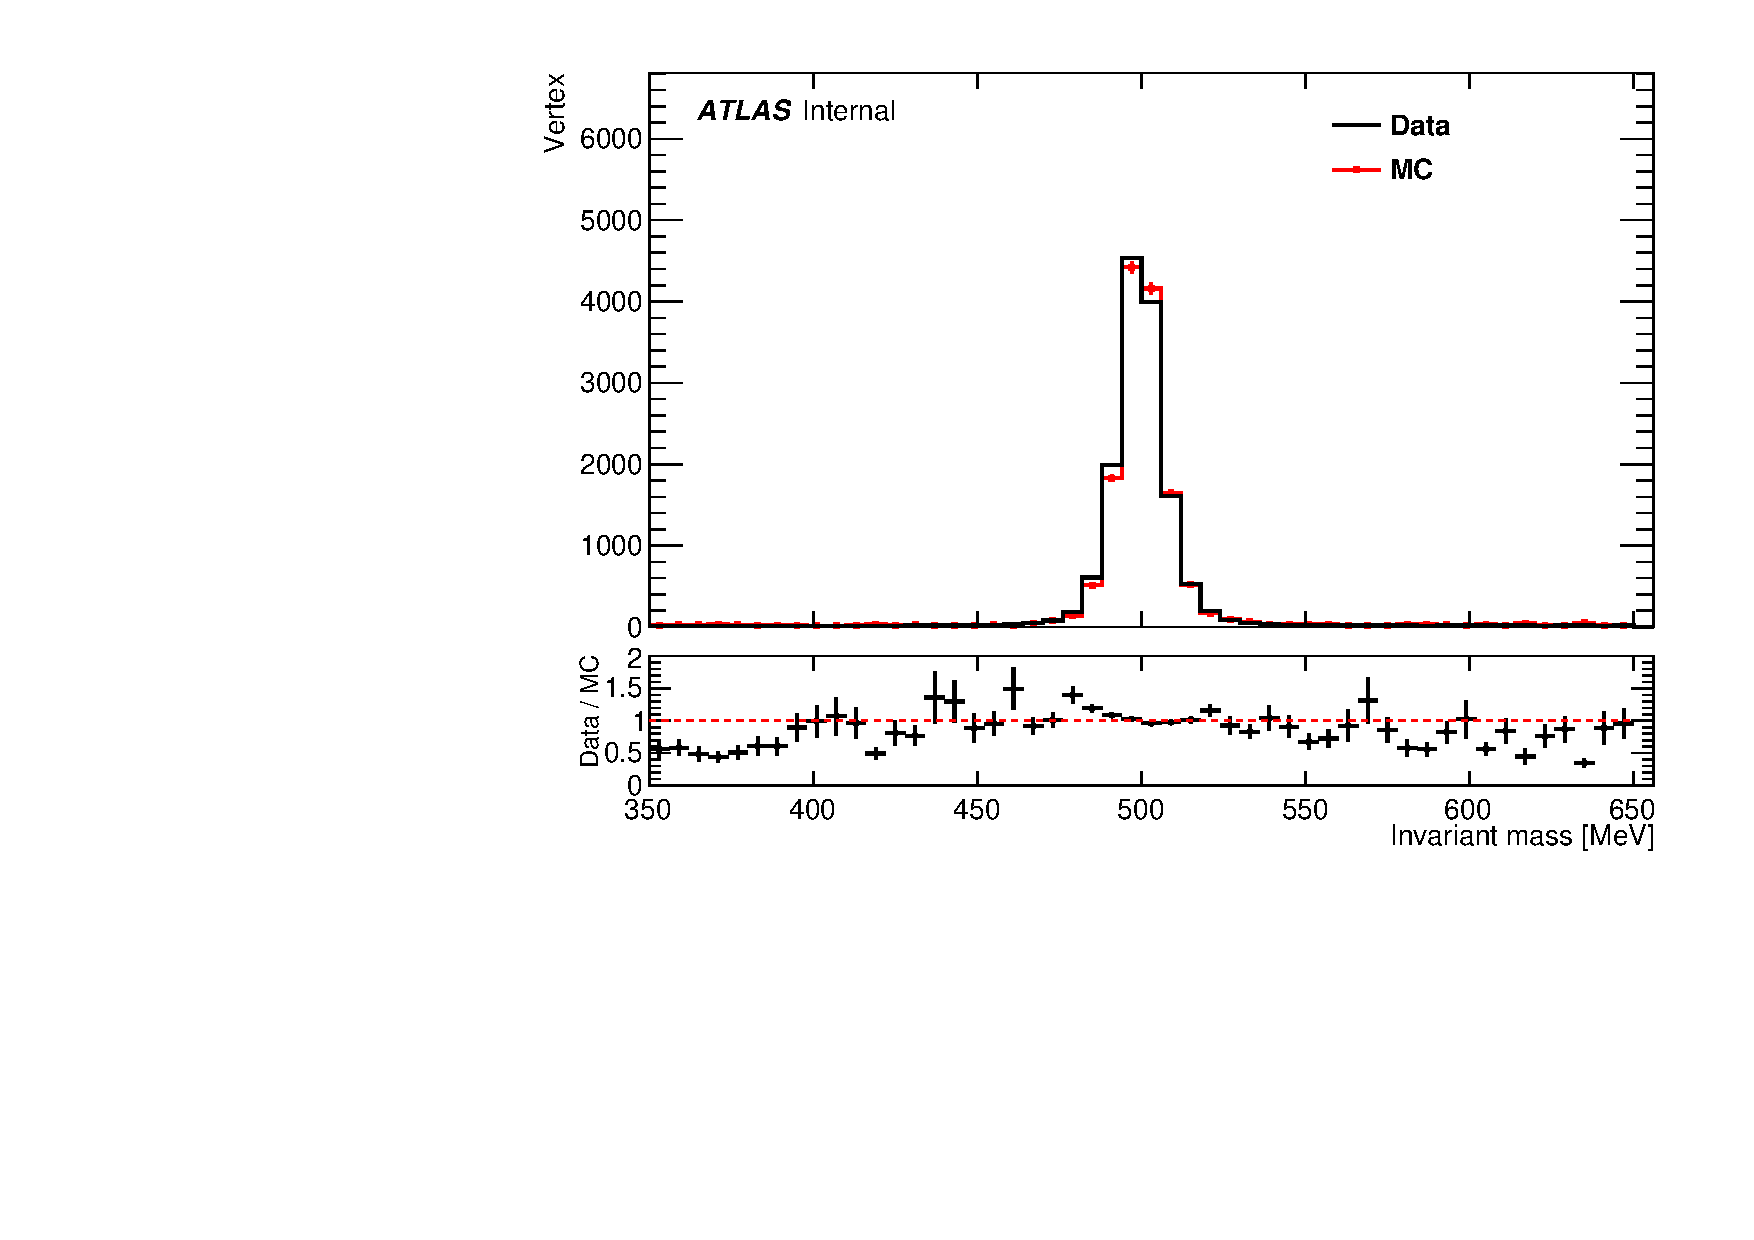
\includegraphics[width=0.45\textwidth]{figures/m_syst_Ks_M.pdf}}
    \subfloat[]{\label{subfig:Ks_pt}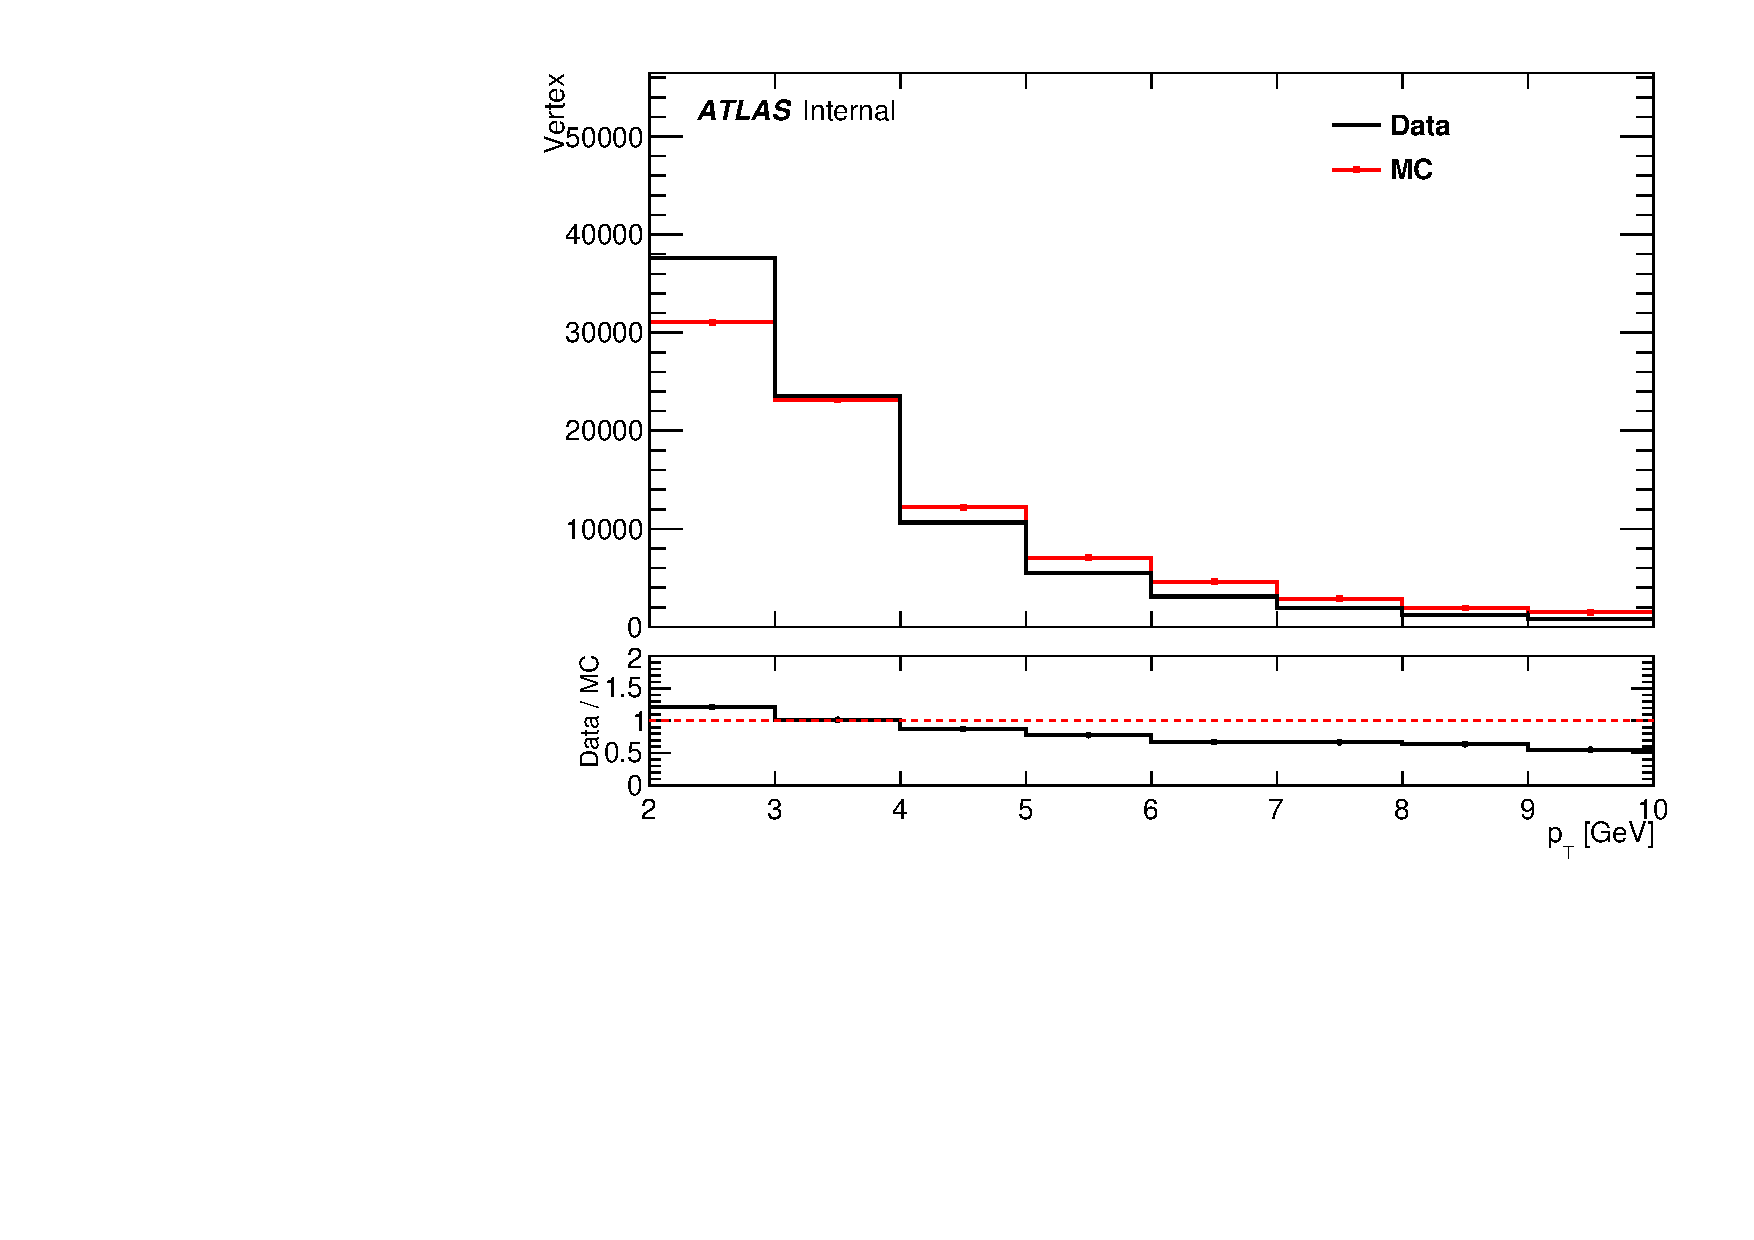
\includegraphics[width=0.45\textwidth]{figures/m_syst_Ks_pt.pdf}} \\
    \subfloat[]{\label{subfig:Ks_mu}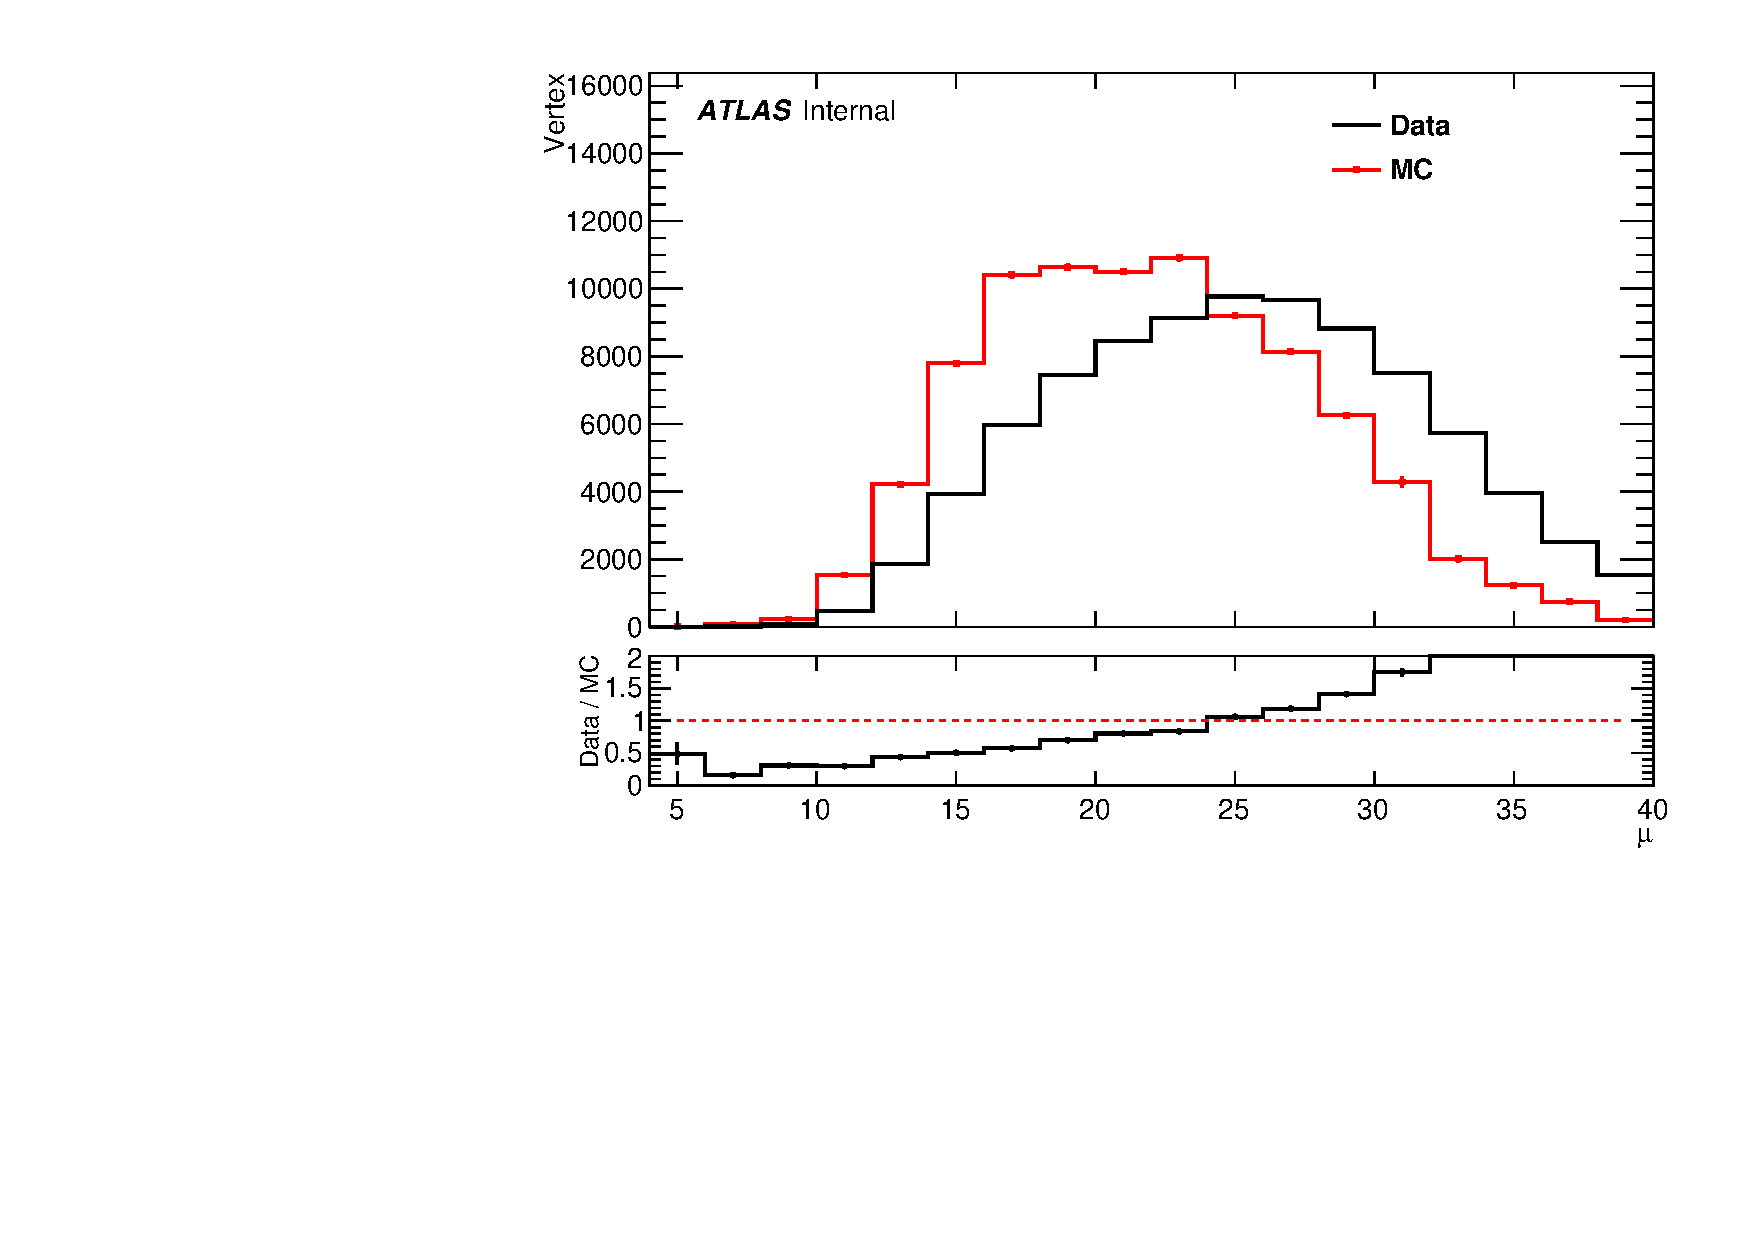
\includegraphics[width=0.45\textwidth]{figures/m_syst_Ks_mu.pdf}}
    \subfloat[]{\label{subfig:Ks_r}\includegraphics[width=0.45\textwidth]{figures/m_syst_Ks_r.pdf}}  \\
    \subfloat[]{\label{subfig:Ks_z}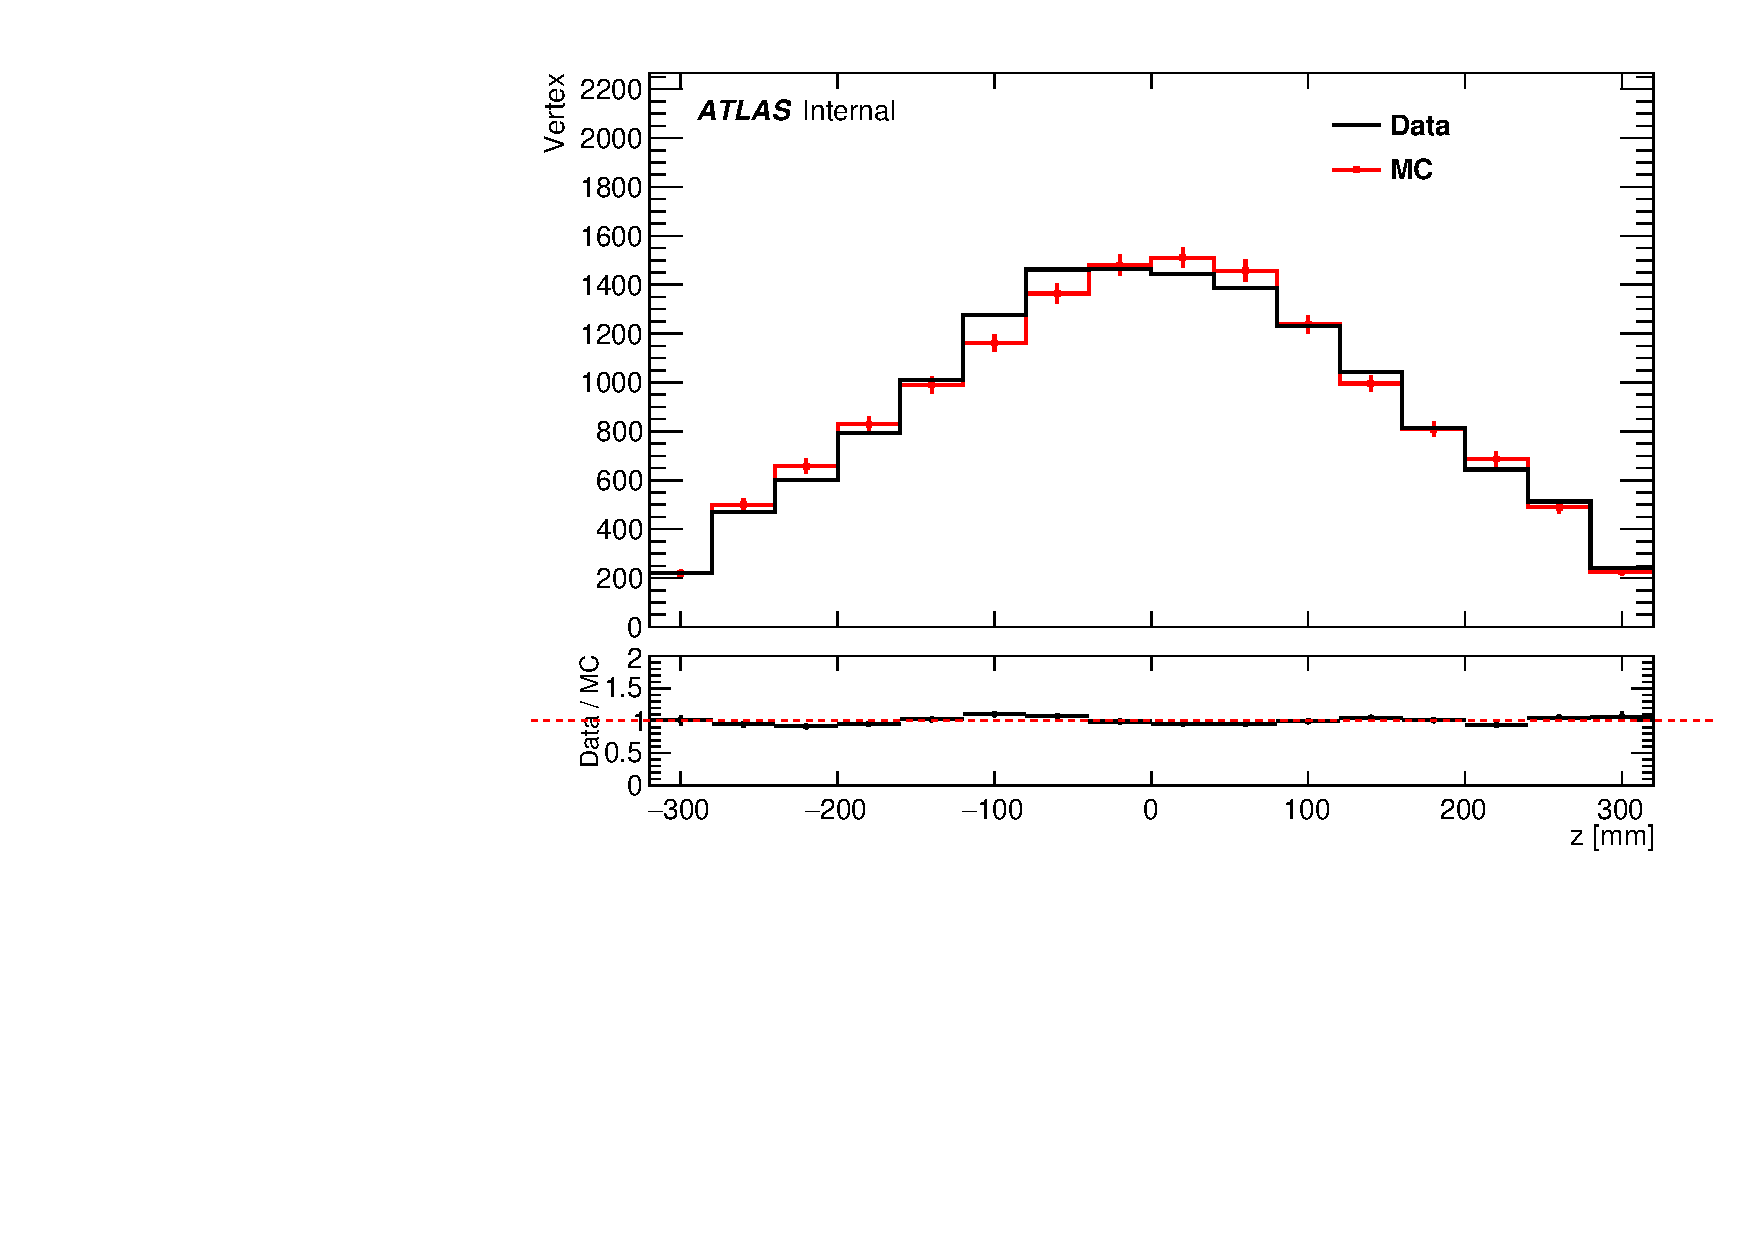
\includegraphics[width=0.45\textwidth]{figures/m_syst_Ks_z.pdf}} 
    \subfloat[]{\label{subfig:Ks_l}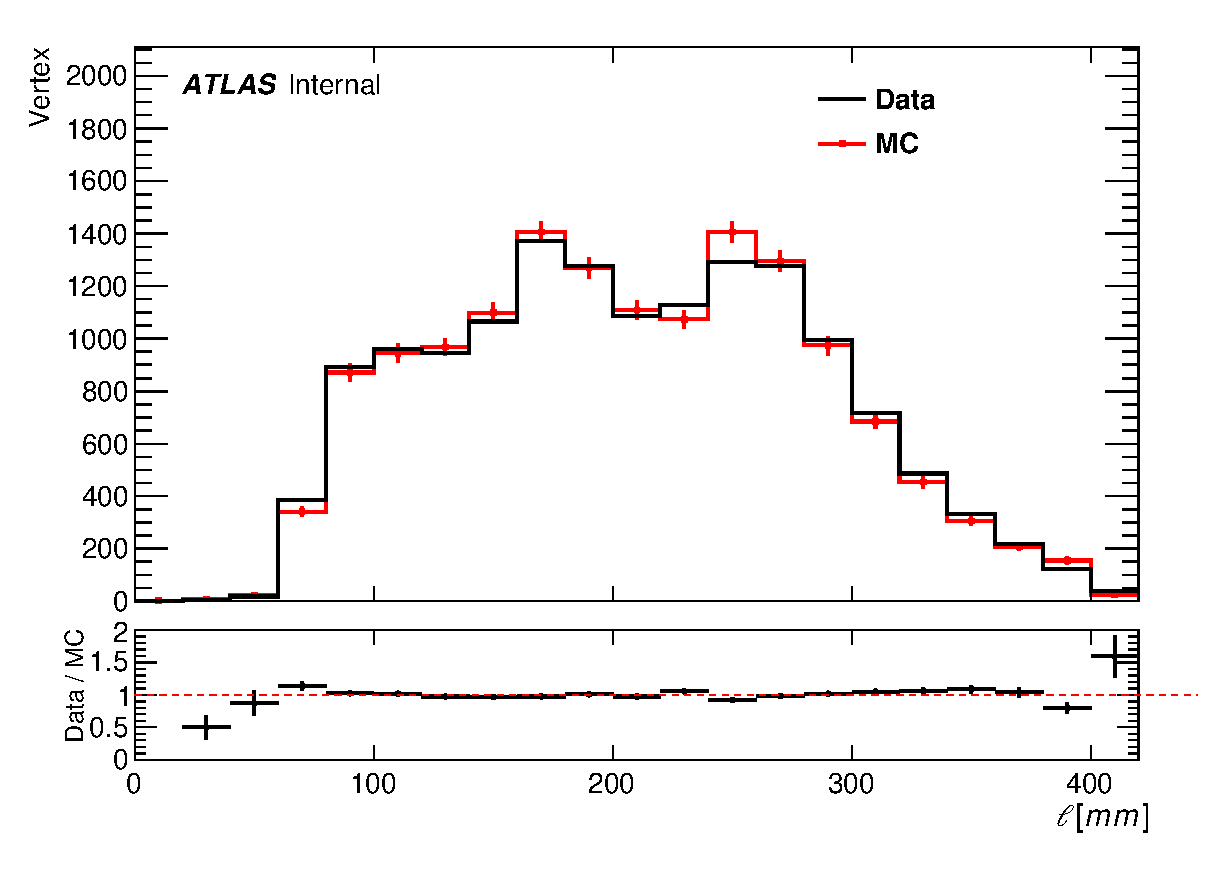
\includegraphics[width=0.45\textwidth]{figures/m_syst_Ks_l.eps}} \\
    \caption{Comparison of the (a) invariant mass, (b) $p_{T}$, (c) $\mu$, (d) transverse, (e) longitudinal position, and (f) decay length of $K_{S}$ with two large-radius tracks in the data with the MC samples. Data is normalized to MC. In (d), the red dashed lines indicate the four Pixel layers and the first layer of SCT. The green dotted lines indicate the Inner Support Tube (45.5 mm) and Pixel Support Tube (229 mm). MC sample is reweighted to the pile-up distribution in data.}
    \label{fig:Ks_data_MC}
\end{figure}

$K_{S}$ vertices found in the data and the MC samples are binned in decay radius, $r$, and the $K_{S}$ yields in each bin are estimated by subtracting the contributions from side-bands (350-450 GeV, 550-650 GeV) in invariant mass distribution. Figure~\ref{fig:Ks_mass} shows the mass distribution of $K_{S}$ with two large-radius tracks from the data and the MC samples. The figure shows that backgrounds are small and uniform in the mass window, and the mass distributions are in good agreement between the data and the MC samples.

%\begin{figure}[tb]
\begin{figure}[!htb]
    \centering
    \subfloat[]{\label{subfig:Ks_mass1}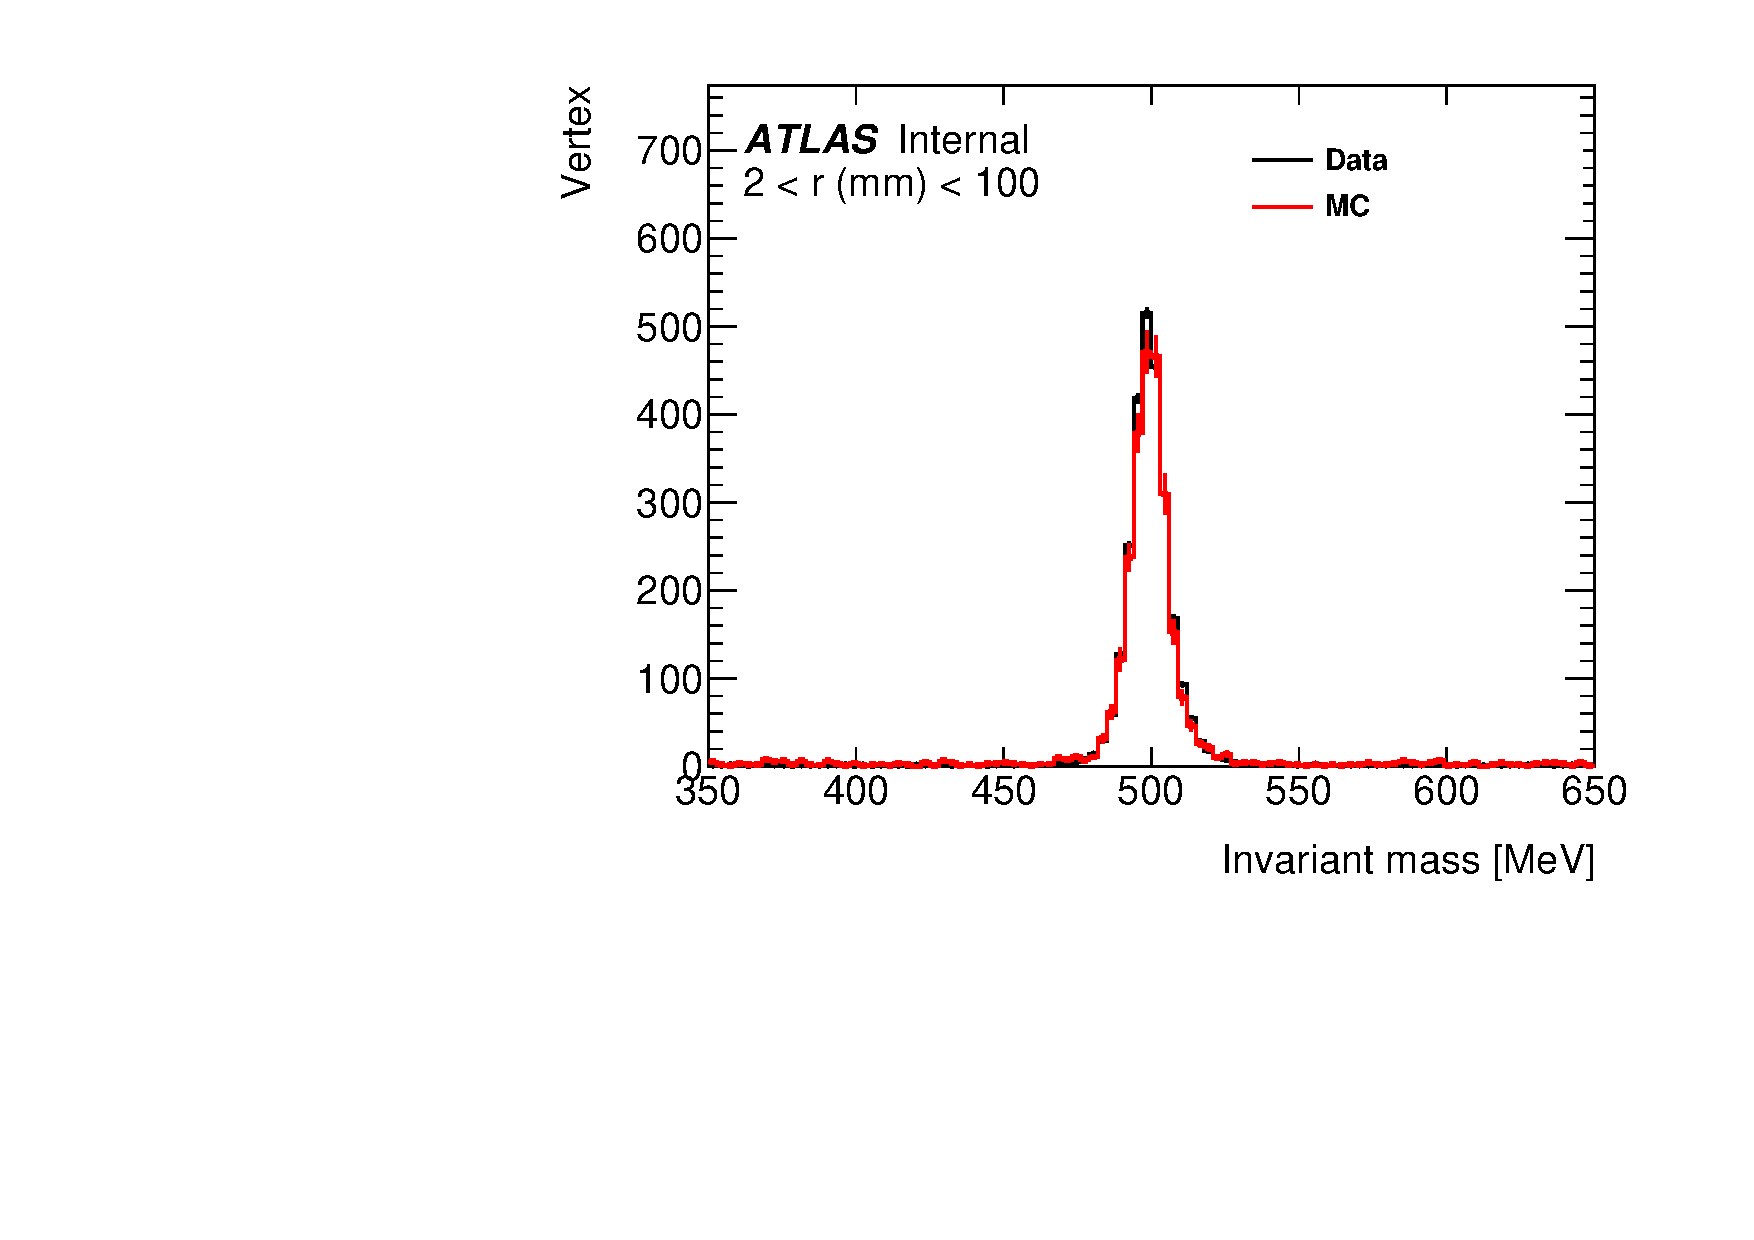
\includegraphics[width=0.45\textwidth]{figures/m_syst_Ks_normalized_LRT_R1.pdf}}
    \subfloat[]{\label{subfig:Ks_mass2}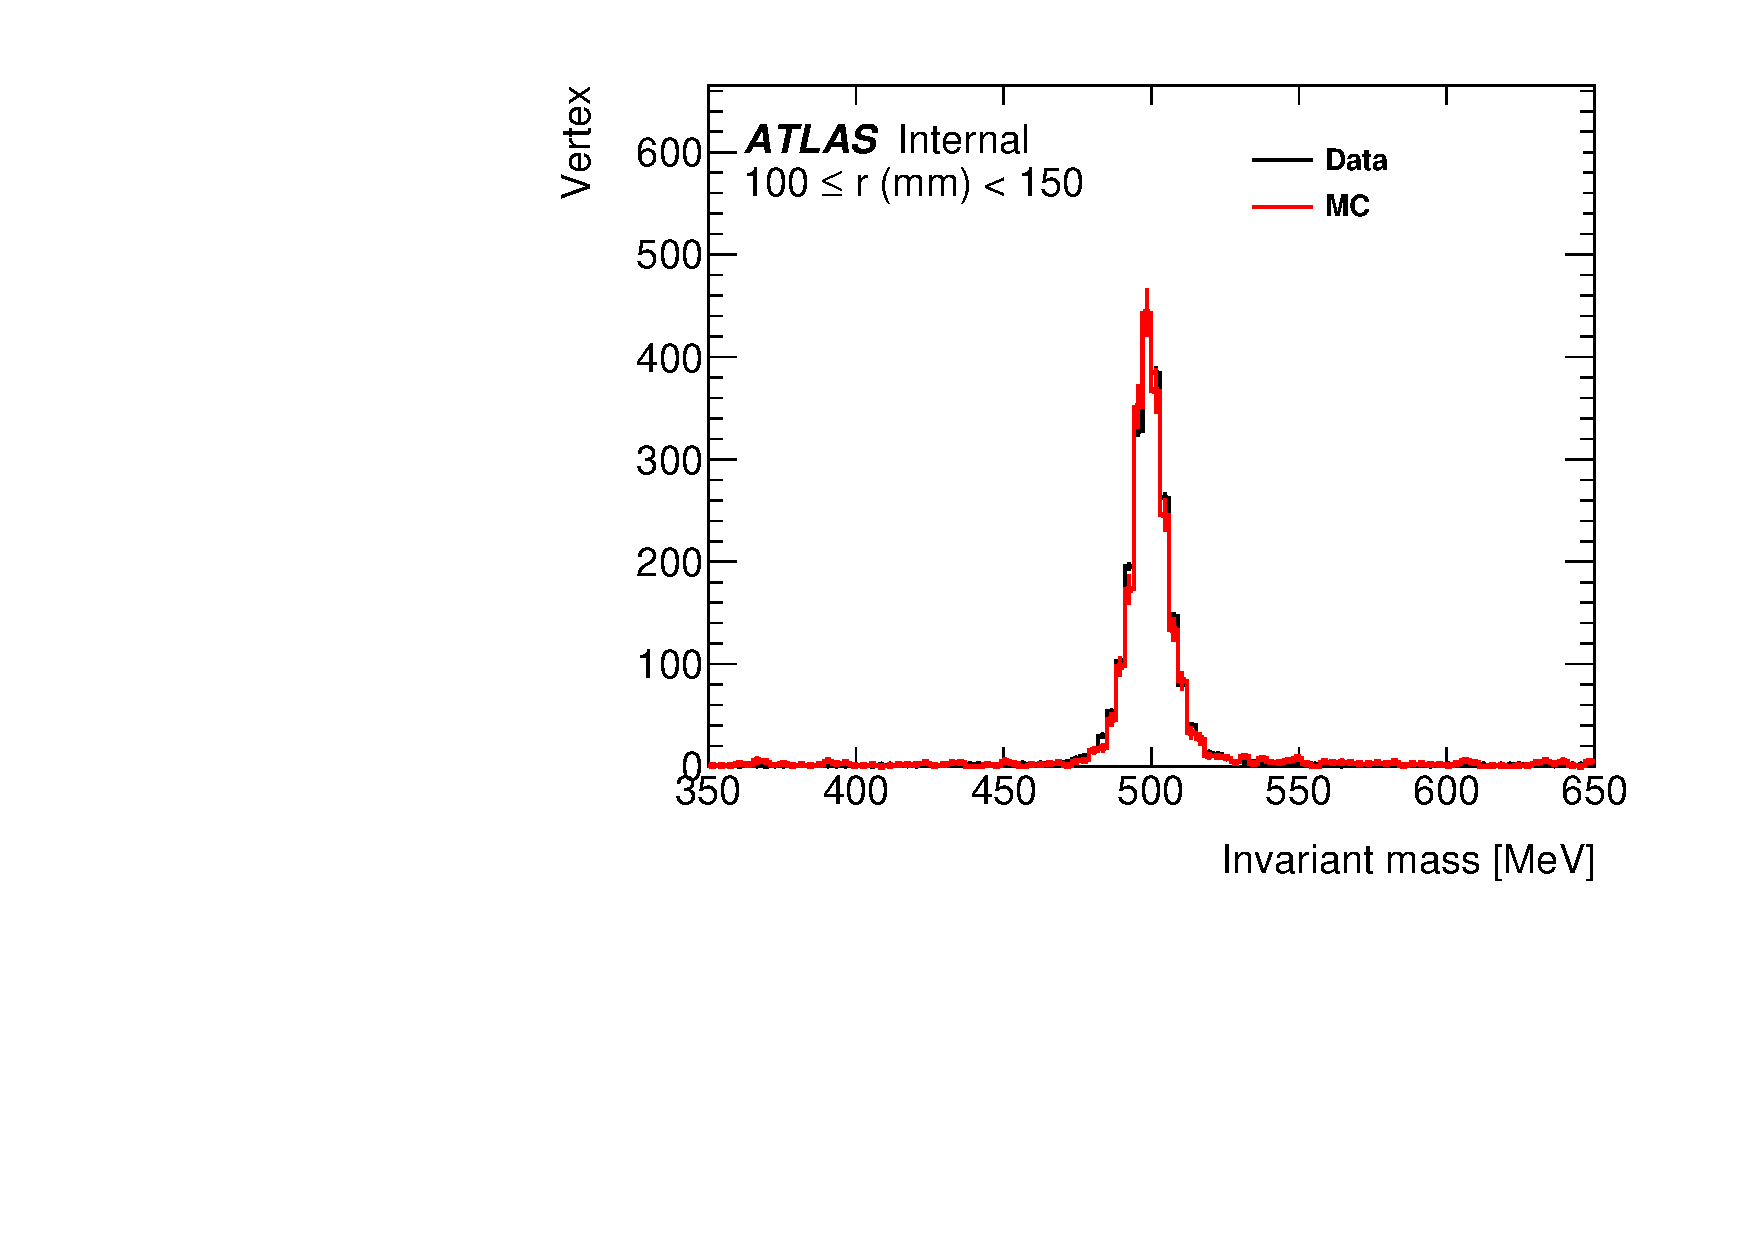
\includegraphics[width=0.45\textwidth]{figures/m_syst_Ks_normalized_LRT_R2.pdf}} \\
    \subfloat[]{\label{subfig:Ks_mass3}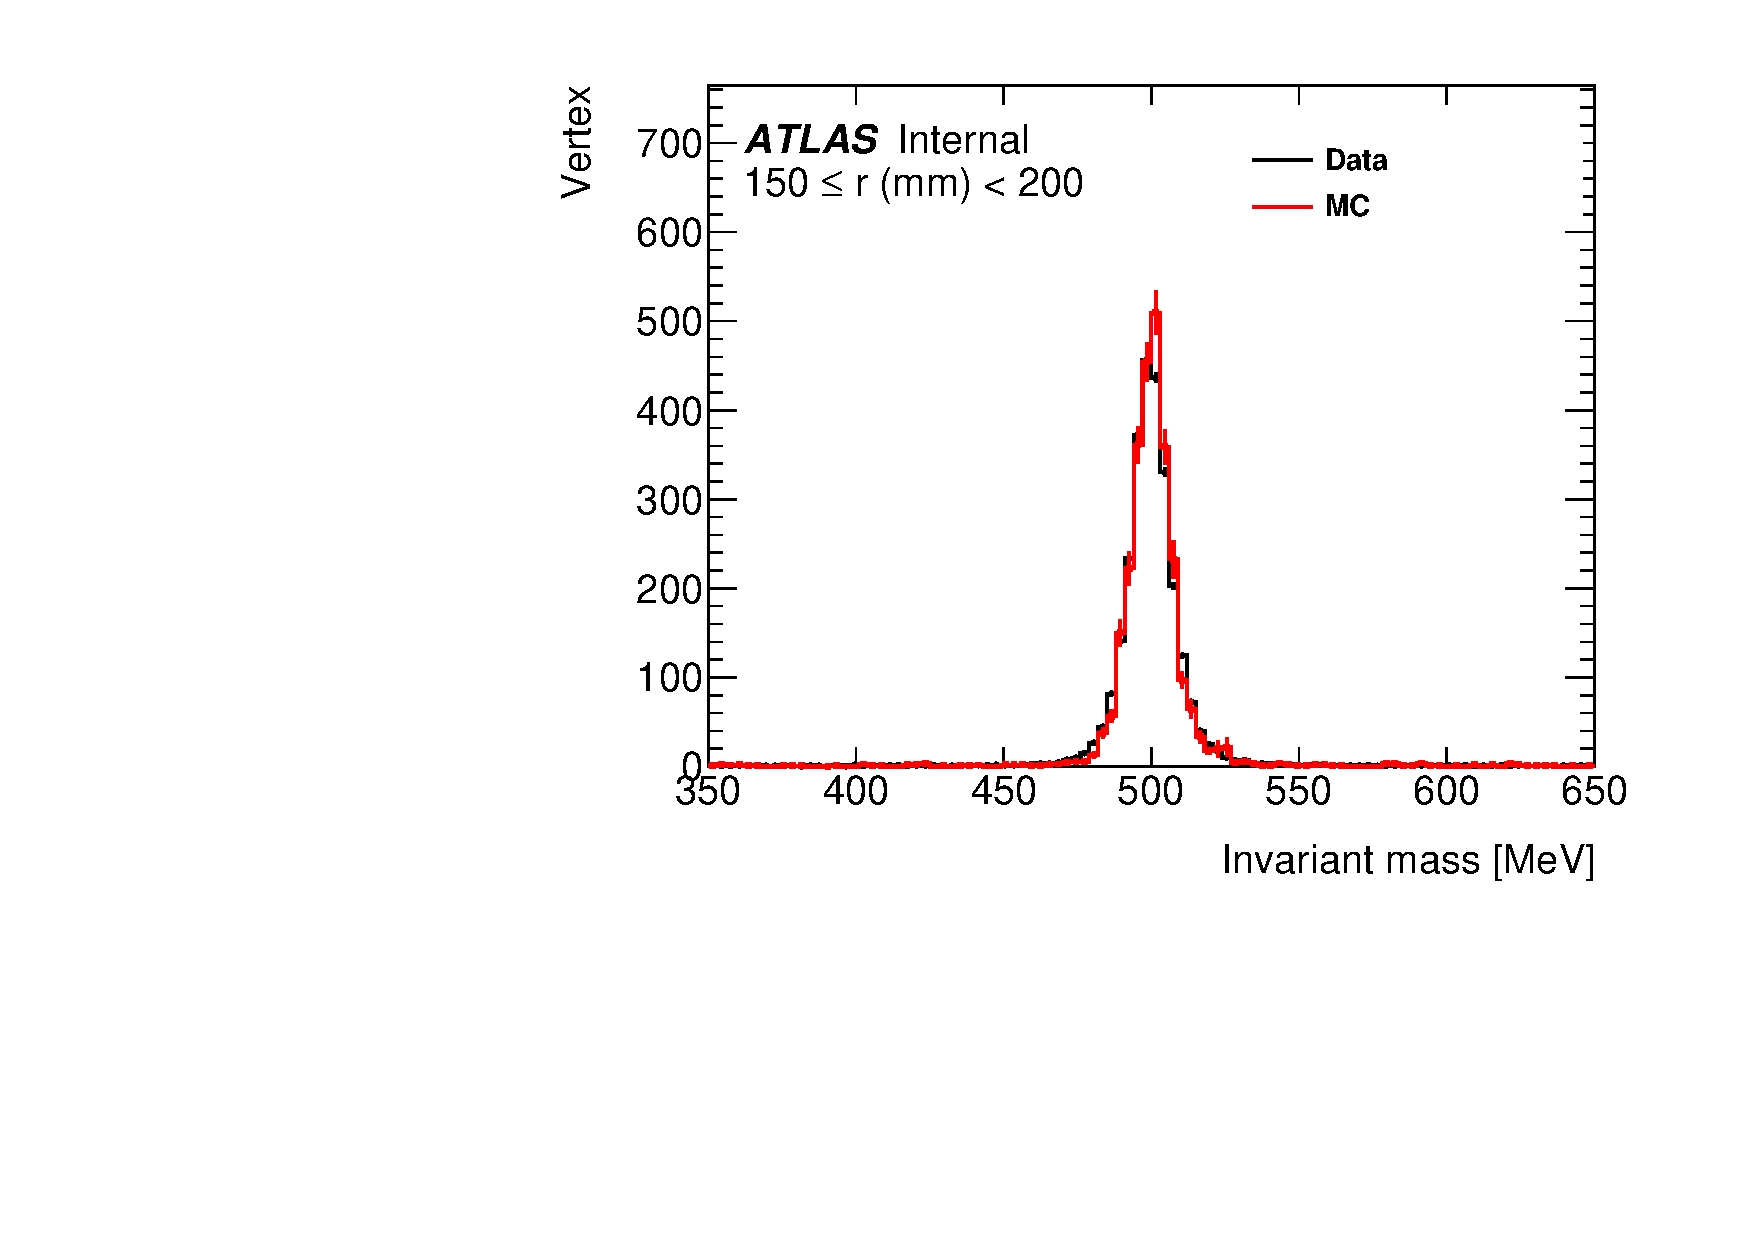
\includegraphics[width=0.45\textwidth]{figures/m_syst_Ks_normalized_LRT_R3.pdf}} 
    \subfloat[]{\label{subfig:Ks_mass4}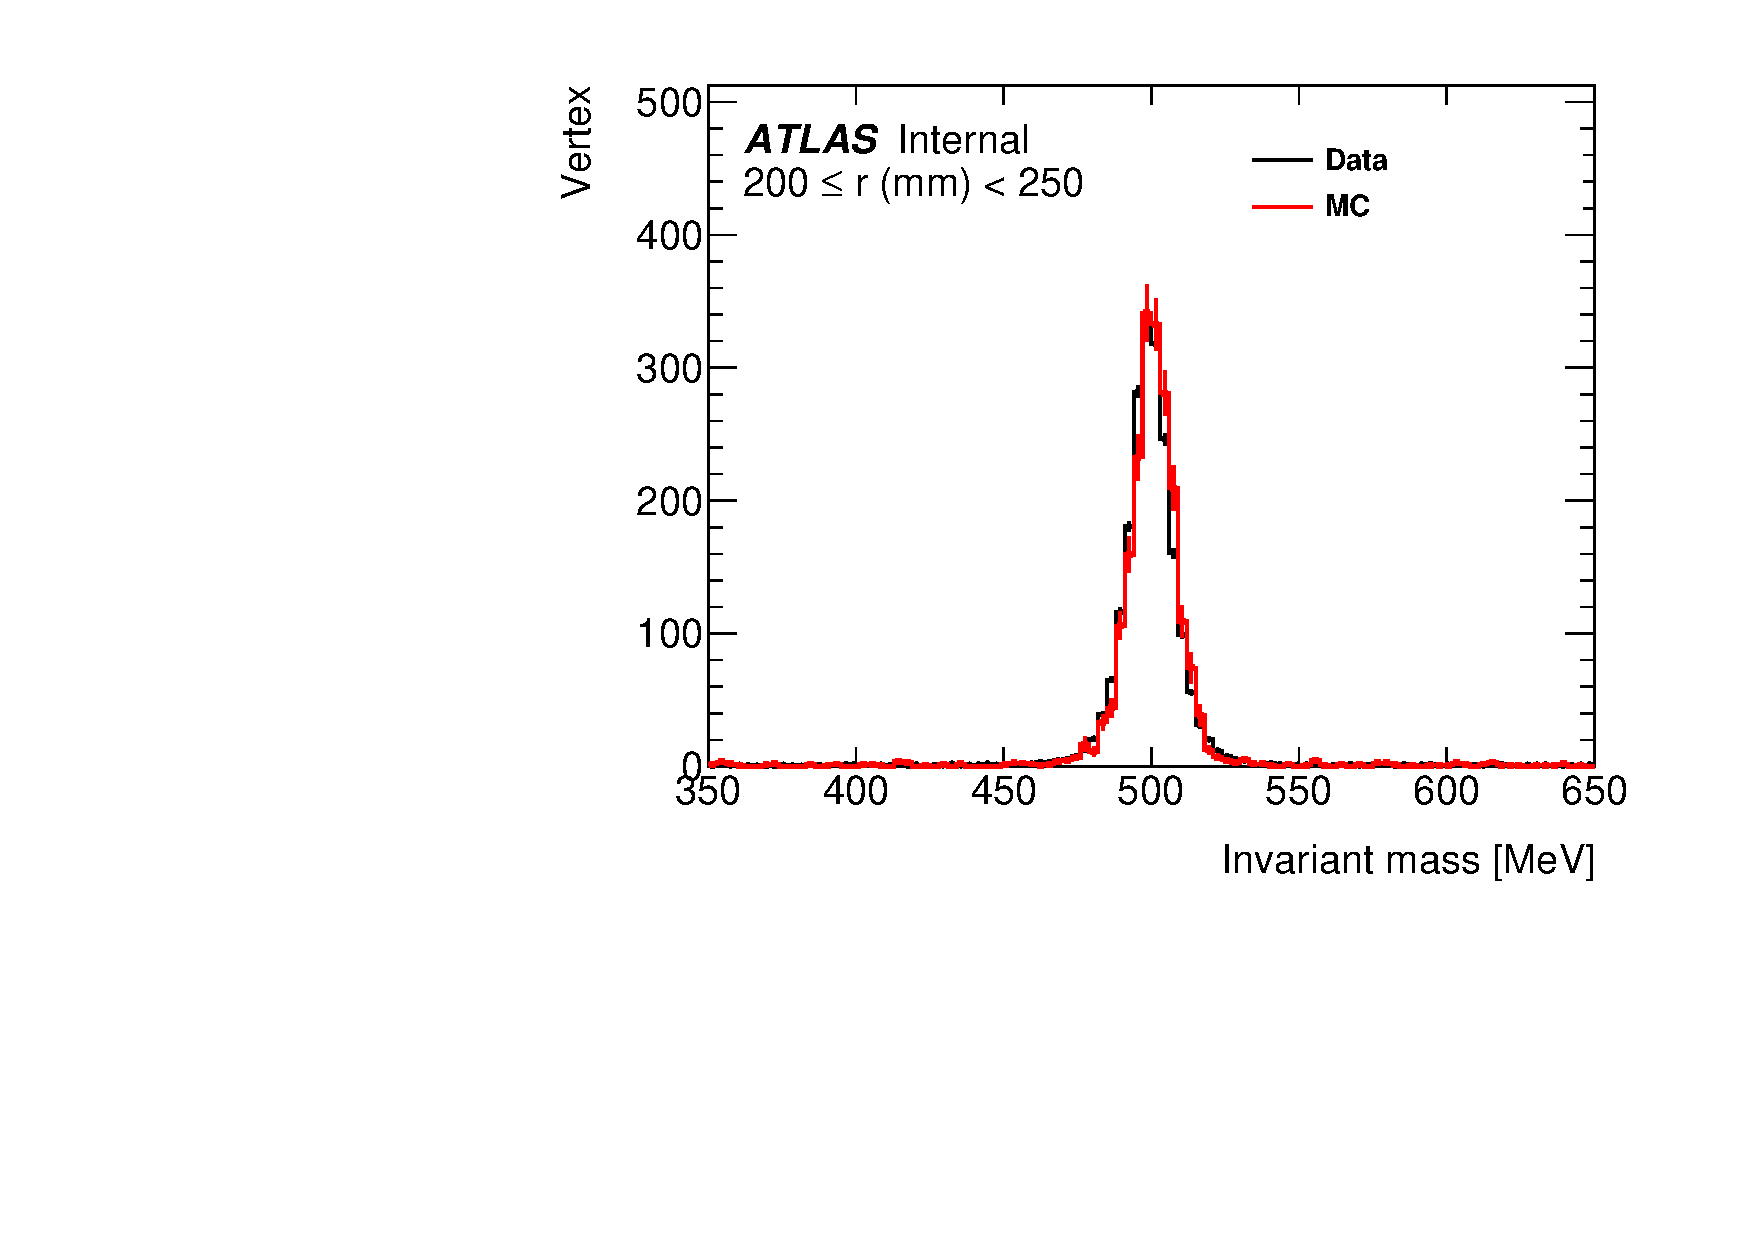
\includegraphics[width=0.45\textwidth]{figures/m_syst_Ks_normalized_LRT_R4.pdf}} \\
    \subfloat[]{\label{subfig:Ks_mass5}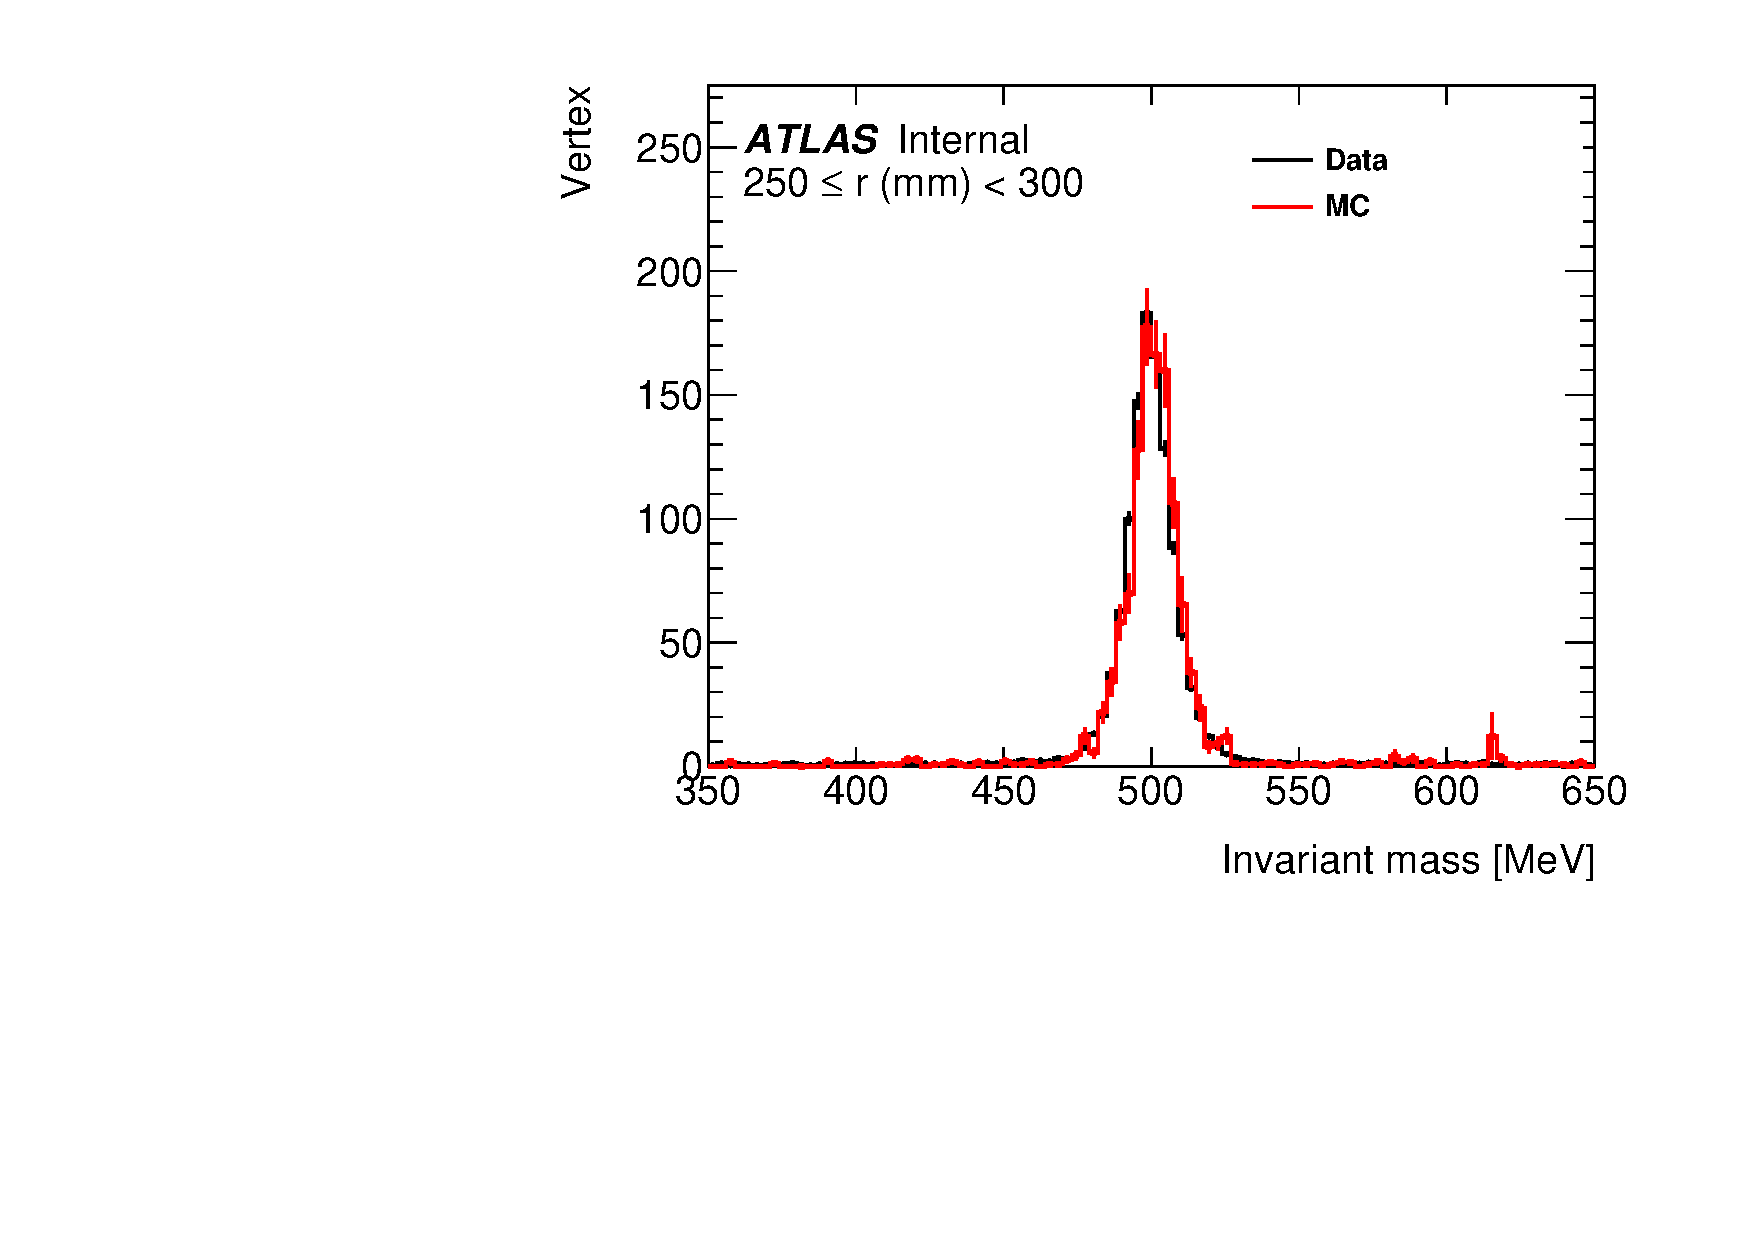
\includegraphics[width=0.45\textwidth]{figures/m_syst_Ks_normalized_LRT_R5.pdf}} 
    \caption{Representative distributions of the invariant mass of $K_{S}$ with two large-radius tracks for (a) 2 < $r$ < 100 mm, (b) 100 $<r<$ 150 mm, (c) 150 $<r<$ 200 mm, (d) 200 $<r<$ 250 mm, and (e) 250 $<r<$ 300 mm in the data and the MC samples. Data is normalized to MC samples.}
    \label{fig:Ks_mass}
\end{figure}

The vertex yields of $K_{S}$ with two large-radius tracks are compared between data and MC samples in Figure~\ref{fig:Ks_double_ratio}, where the data is normalized by a factor of $N_{\mathrm{ST}} / N_{\mathrm{ST}}^{\mathrm{MC}}$ where $N_{\mathrm{ST}}$ and $N_{\mathrm{ST}}^{\mathrm{MC}}$ are integrated over $r$. The ratio between two, representing the double ratio (Eq.~\ref{eq:Ks_eq2}), is shown in the lower pane.

\begin{figure}[!htb]
	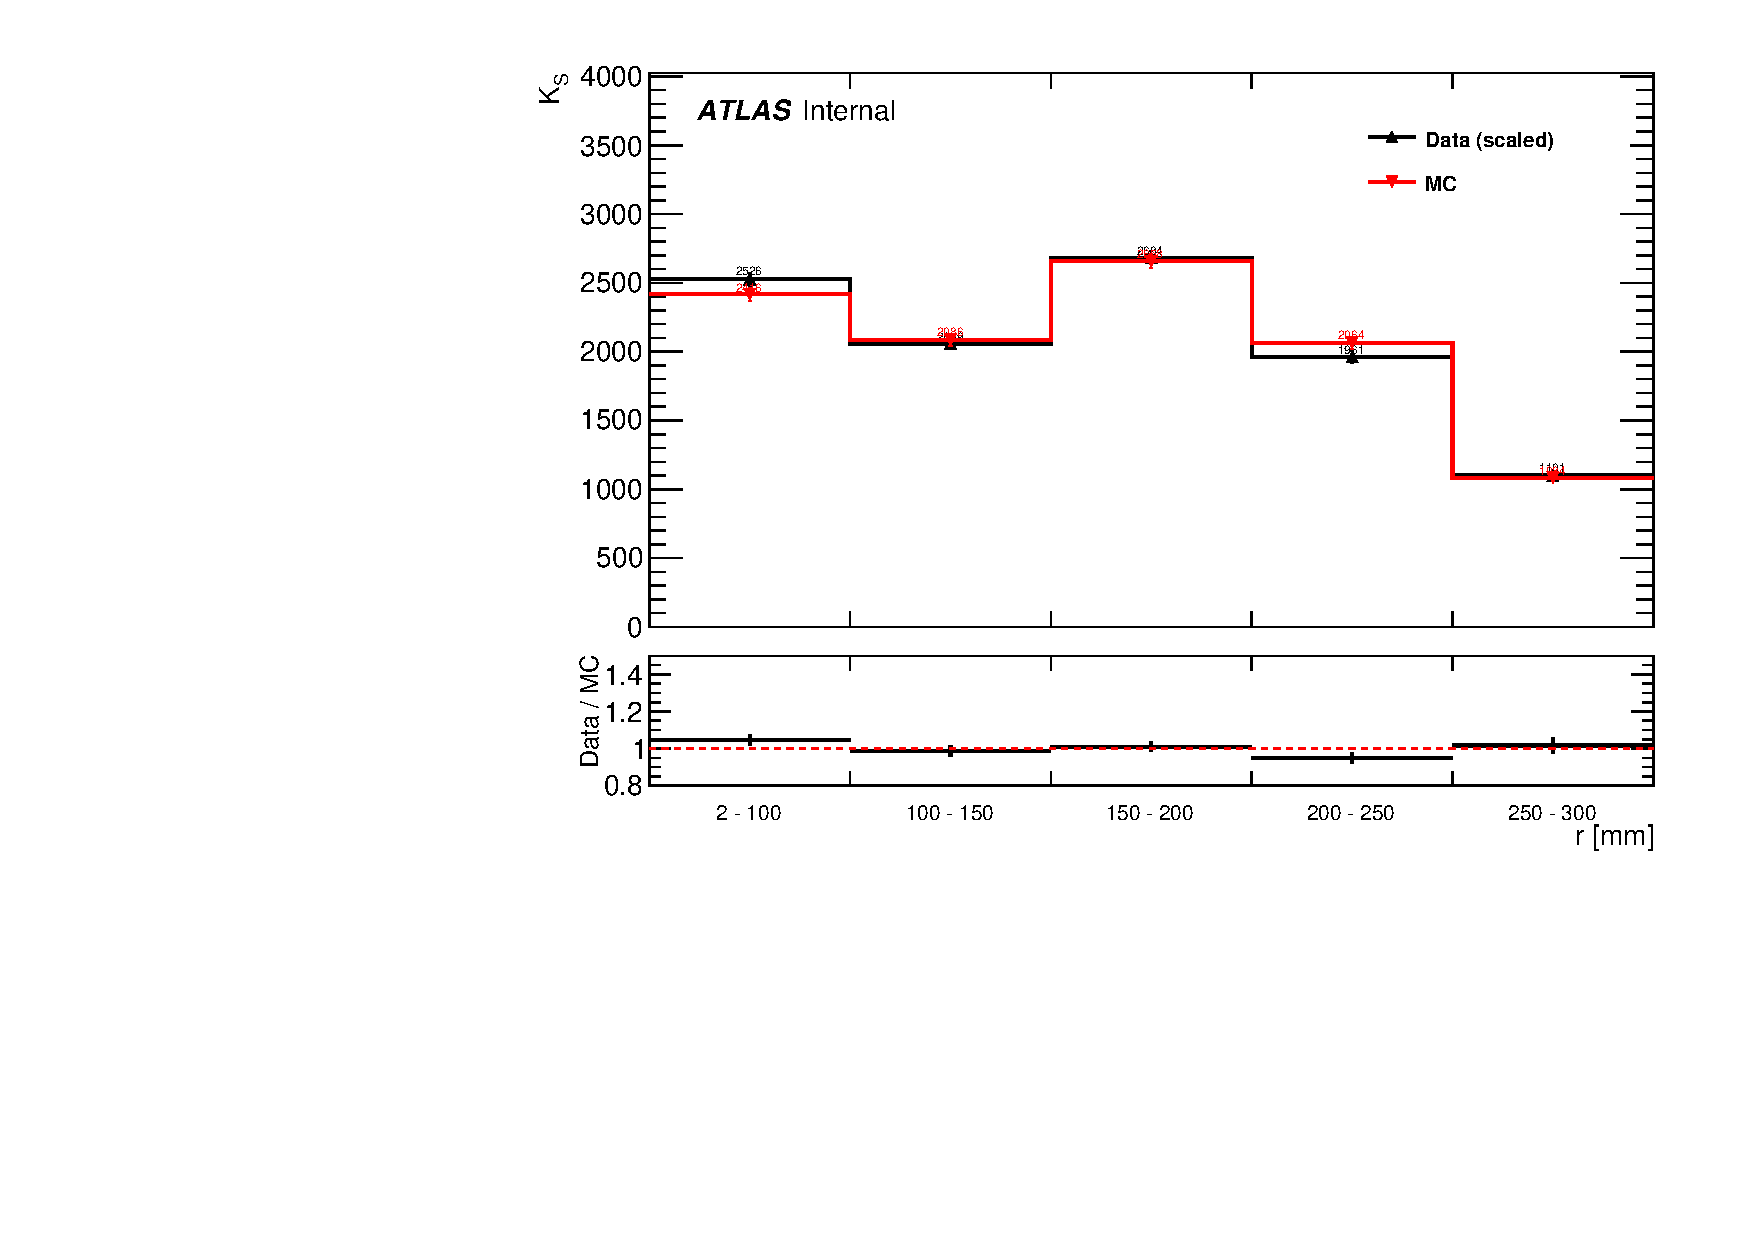
\includegraphics[width=0.50\textwidth]{figures/m_syst_Ks_ratio_R.pdf}
	\centering
	\caption{The radial distribution of vertex yields of $K_{S}$ with two large-radius tracks. Data is normalized by the ratio of vertex yield of $K_{\mathrm{ST}}$ in data to the corresponding vertex yields in MC. The lower pane shows the double ratio defined in Eq.~\ref{eq:Ks_eq2}.}
	\label{fig:Ks_double_ratio}
\end{figure}

In estimating the systematic uncertainty, largest discrepancies ($\sim0.95$, and $\sim1.05$), shown in the first and fourthbin, are taken as a conservative estimate. The results from previous studies show that the systematic uncertainty in the standard tracking is $2\%$~\cite{ATL-PHYS-PUB-2015-051}, and the systematic uncertainty in secondary vertex reconstruction using standard tracks is $1\%$~\cite{Aaboud:2215485}. Using Eq.~\ref{eq:Ks_eq3} together with these results, the systematic uncertainty in track and vertex reconstruction in the LRT is estimated to be $10\%$.




















\section{Systematic Uncertainties in Trigger Efficiency}
\label{sec:syst:trigger}

Systematic uncertainties in lepton triggers are usually measured with tag-and-probe studies on $Z$+jet where most leptons have small impact parameters. However, because the leptons originating from displaced vertices tend to have large impact parameters, the standard systematics on triggers provided by the performance groups cannot be applied. In the following, the systematic uncertainties in the lepton triggers are estimated using tag-and-probe method on the data and $Z$+jets MC samples. 

The estimated systematic uncertainties are valid only if the trigger efficiencies do not depend on impact parameters or if this dependence is modelled reasonable well in simulations. Therefore, the efficiencies of the single photon and single muon triggers listed on Table~\ref{table:triggers} are estimated using the signal MC samples and shown in Figure~\ref{fig:signal_TrigEff}.

The photon trigger efficiency is consistent for both the transverse and the longitudinal impact parameter. The muon trigger efficiency starts to decrease for large impact parameters, $|\dzero| \sim120~\si{\mm}$ and $|\zzero| \sim200~\si{\mm}$. However, the decreasing muon efficiency at very large impact parameters is neglected since the fraction of reconstructed muons with such large impact parameters is less than 10\% at the lifetime of $c\tau=100~\si{\mm}$.


\begin{figure}[!htp]
    \centering
    \subfloat[]{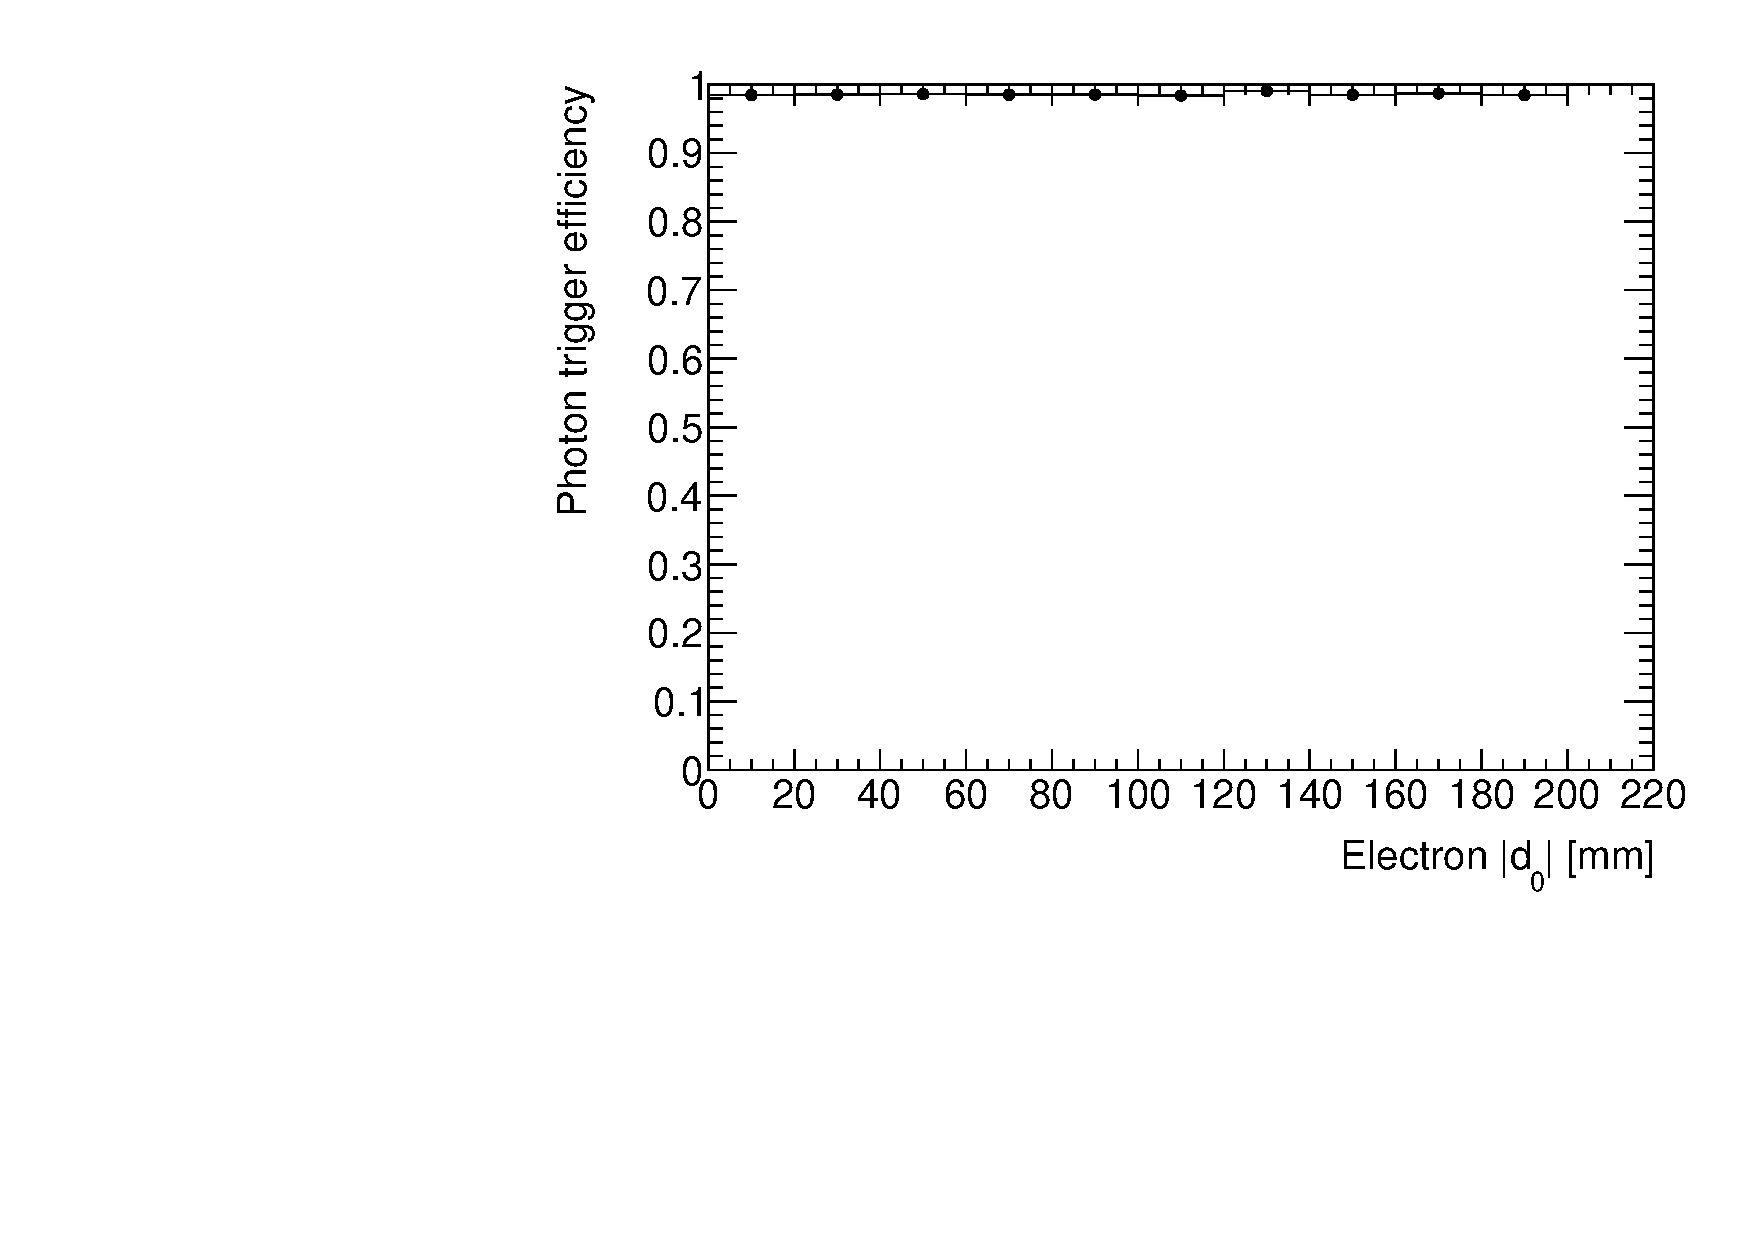
\includegraphics[width = 0.44 \textwidth]{figures/TrigEff/signal/eff_siph_d0.pdf}}
    \subfloat[]{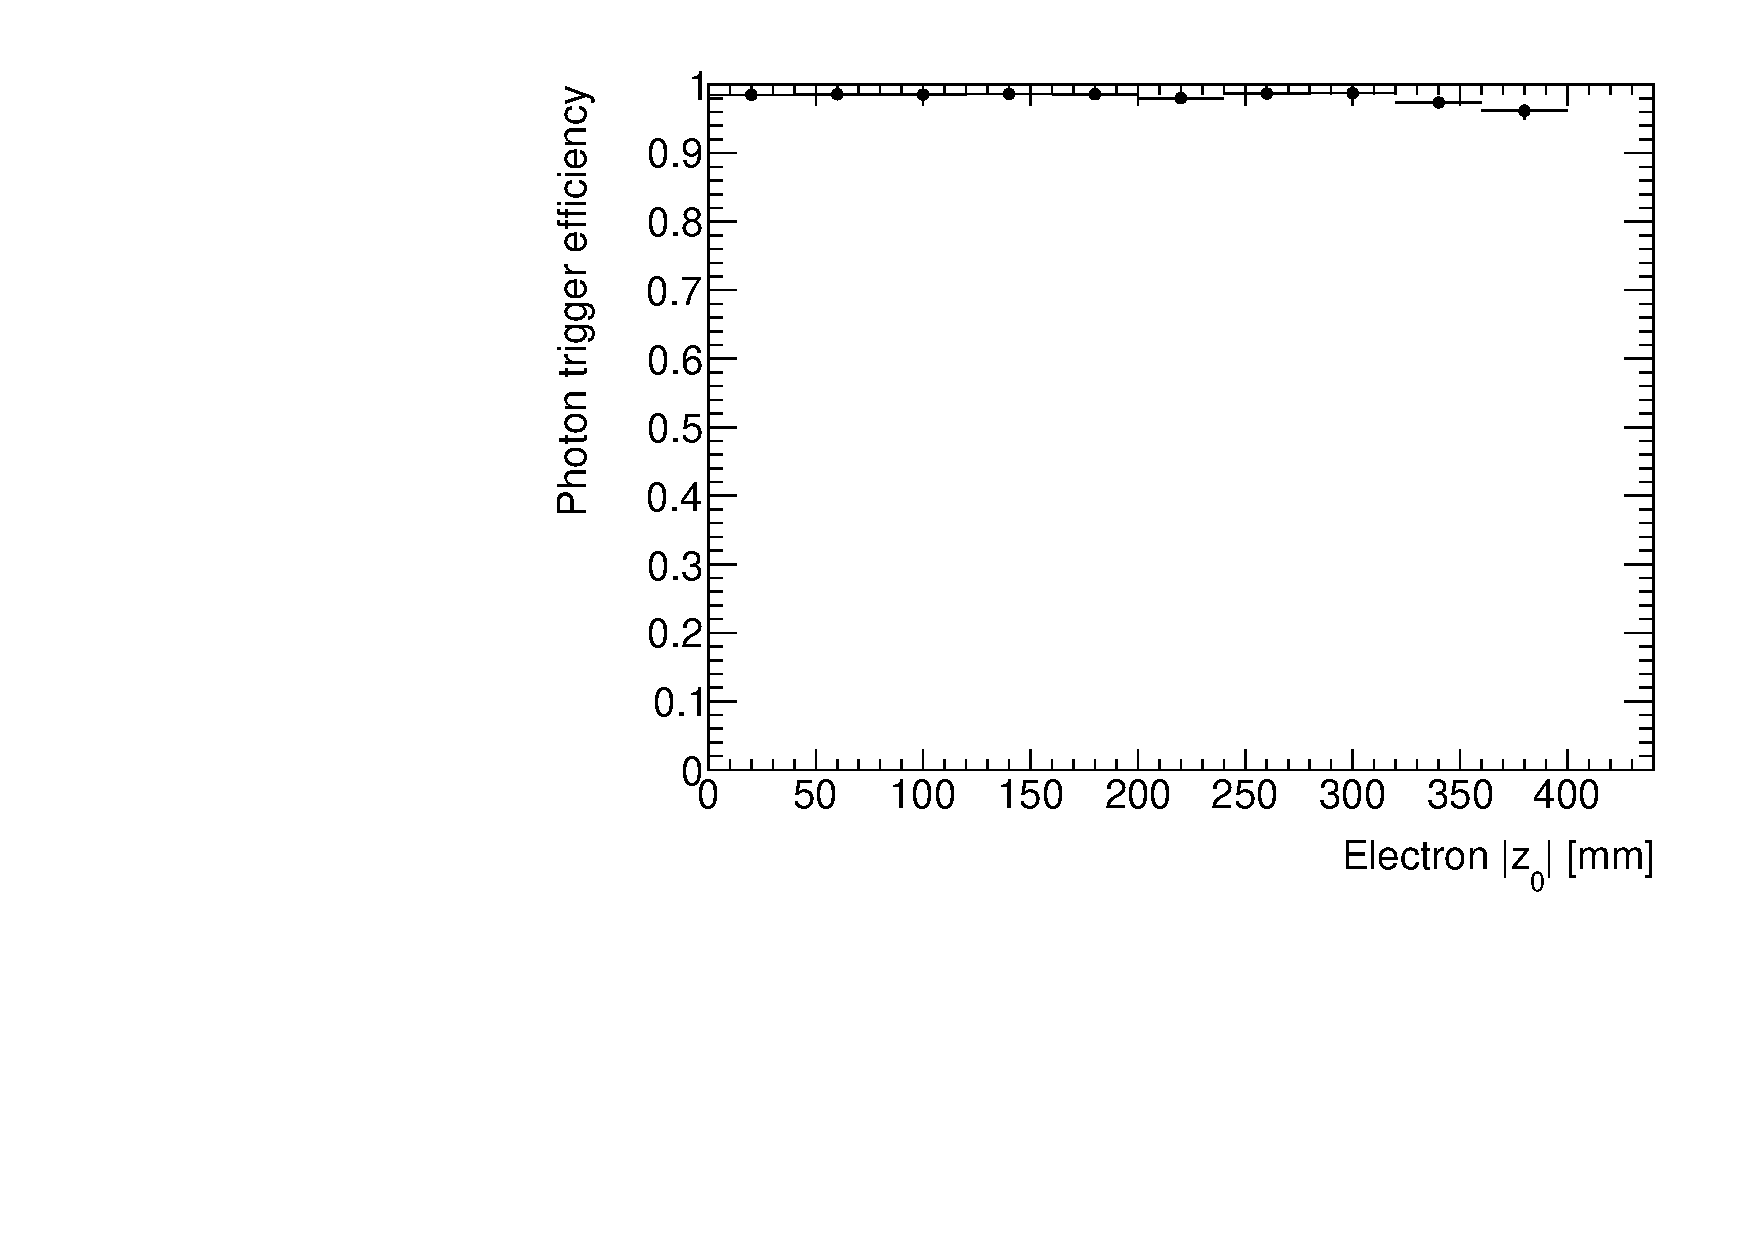
\includegraphics[width = 0.44 \textwidth]{figures/TrigEff/signal/eff_siph_z0.pdf}} \\
    \subfloat[]{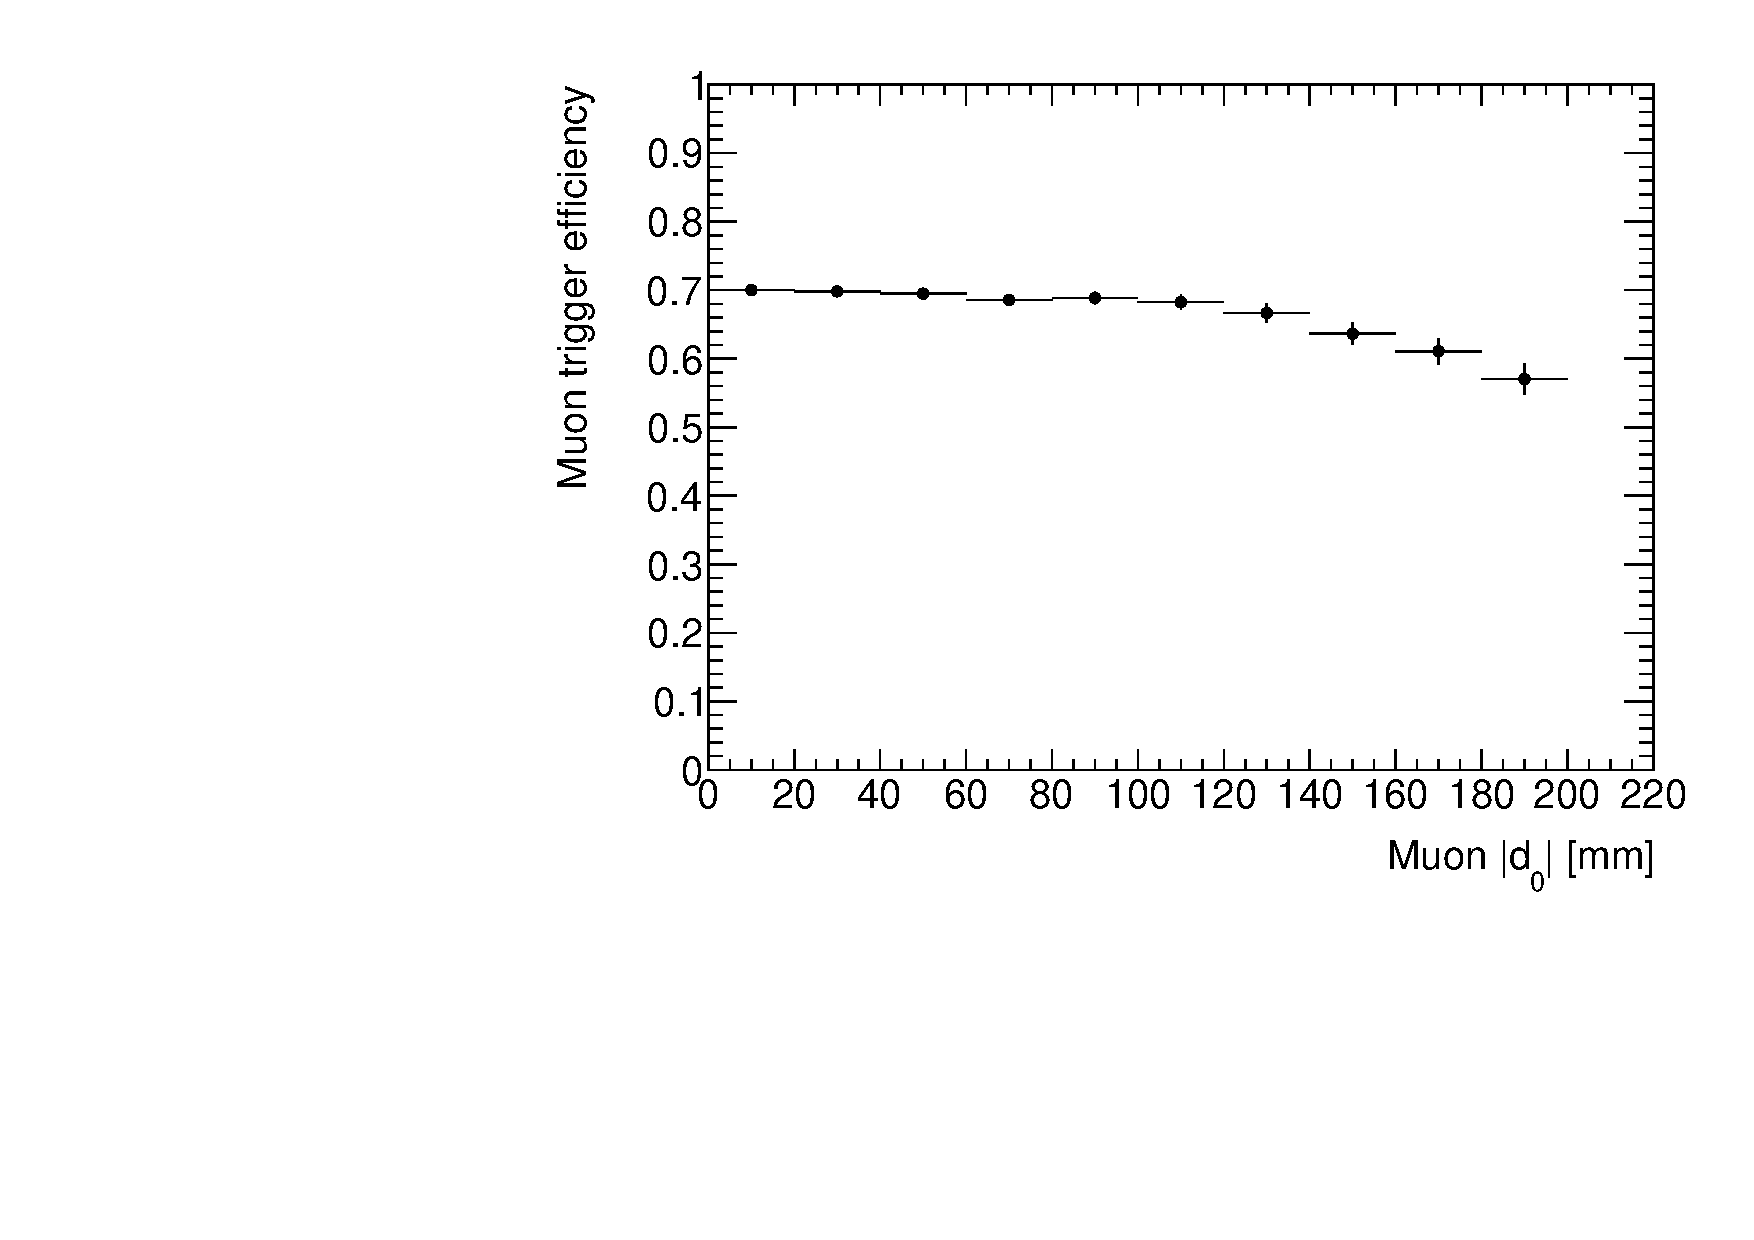
\includegraphics[width = 0.44 \textwidth]{figures/TrigEff/signal/eff_simu_d0.pdf}}
    \subfloat[]{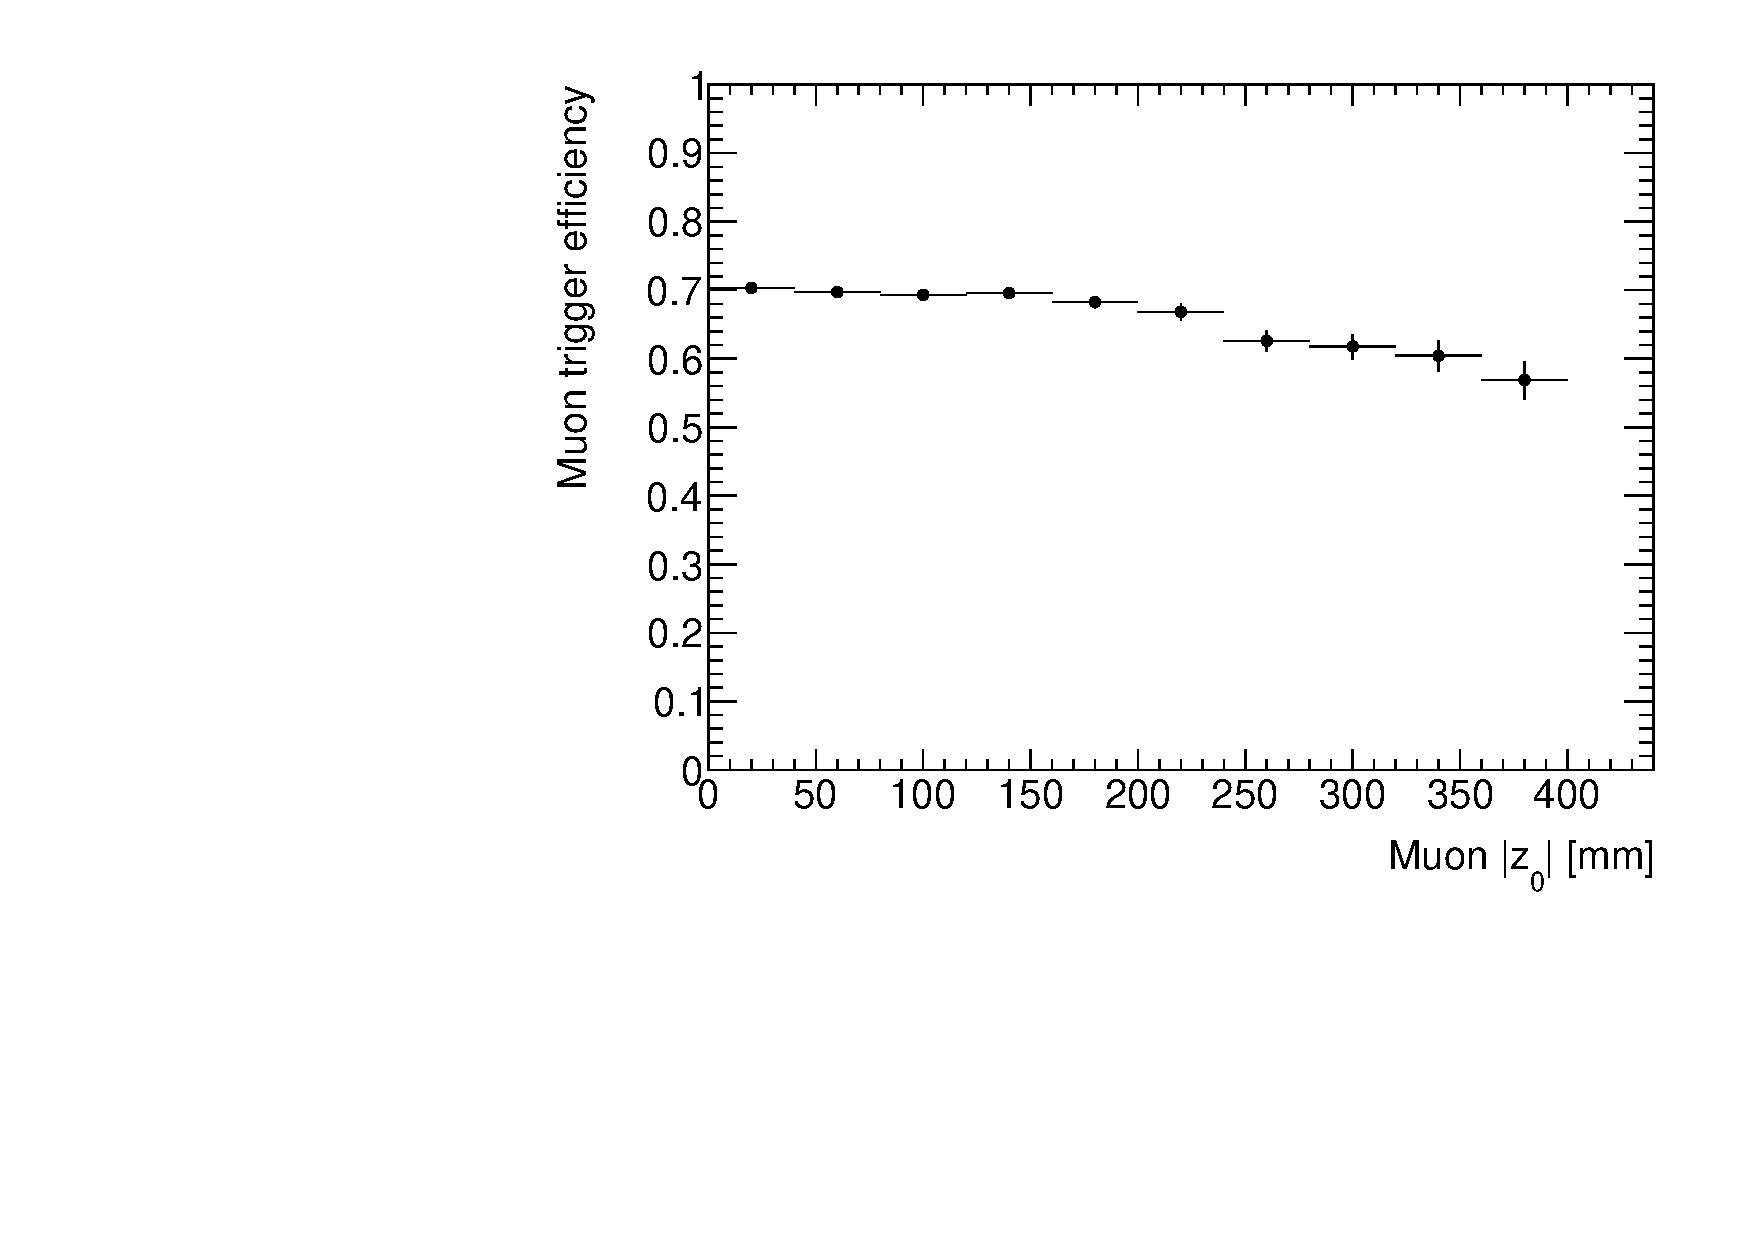
\includegraphics[width = 0.44 \textwidth]{figures/TrigEff/signal/eff_simu_z0.pdf}}
    \caption{The efficiency of the single photon trigger in electron (a) $|\dzero|$ and (b) $|\zzero|$. The corresponding plots of the single muon trigger are shown in (c) and (d).}
    \label{fig:signal_TrigEff}
\end{figure}



\subsection{Photon triggers}
\label{subsect:photonTrigEff}

The systematic uncertainties of the single photon and the di-photon triggers are estimated with a standard tag and probe method on $Z\rightarrow ee$ events both in data and MC samples. The di-photon trigger (\texttt{HLT\_2g50\_loose}) is studied using the single muon trigger (\texttt{HLT\_g50\_loose}) with the same $p_{T}$ threshold. The selection criteria of electron tag-and-probe candidates are listed in Table~\ref{tab:ZeeSelection}. In addition, pairs are required to have opposite signs and to satisfy the mass requirement ($|m_{e^{+}e^{-}} - m_{Z}| < 10~\si{\GeV}$) and the isolation requirement of $\DeltaR(\mathrm{tag}, \mathrm{probe}) > 0.4$. 

\begin{table}[!htb]
	\centering
	\begin{tabular}{ccc}
		\hline
		\hline
		Selection & Tag & Probe \\
		\hline
		$p_{T}$ (GeV) $>$ & 27 & 30 \\
		Trigger matched & \texttt{HLT\_e26\_lhtight\_nod0\_ivarloose} & --- \\
		$|\eta|$ & $<$ 1.37 or ($>$ 1.52 and $<$ 2.47) & < 2.47 \\
		Identification & TightLH & LooseLHNoD0 \\
		Object quality & yes & yes \\
		Track isolation & yes & --- \\
		Jet veto & --- & yes \\
		\hline
		\hline
	\end{tabular}
	\caption{Selection criteria for tag-and-probe electrons in $Z$+jets studies.}
	\label{tab:ZeeSelection}
\end{table}

The invariant mass distributions of the tag-and-probe pairs found in the data and the MC samples are shown in Figure~\ref{fig:PhotonTrigMass}. The shape of distribution is in good agreement with negligible background for both triggers. Therefore, no background subtraction is performed in the calculation of the trigger efficiencies, 

\begin{equation}
	\label{eq:TrigEff}
    \epsilon_{\mathrm{trigger}} = \frac{\textrm{Number of probes matched to trigger}}{\textrm{Number of all probes}}.
\end{equation}

\begin{figure}[!htb]
    \centering
    \subfloat[]{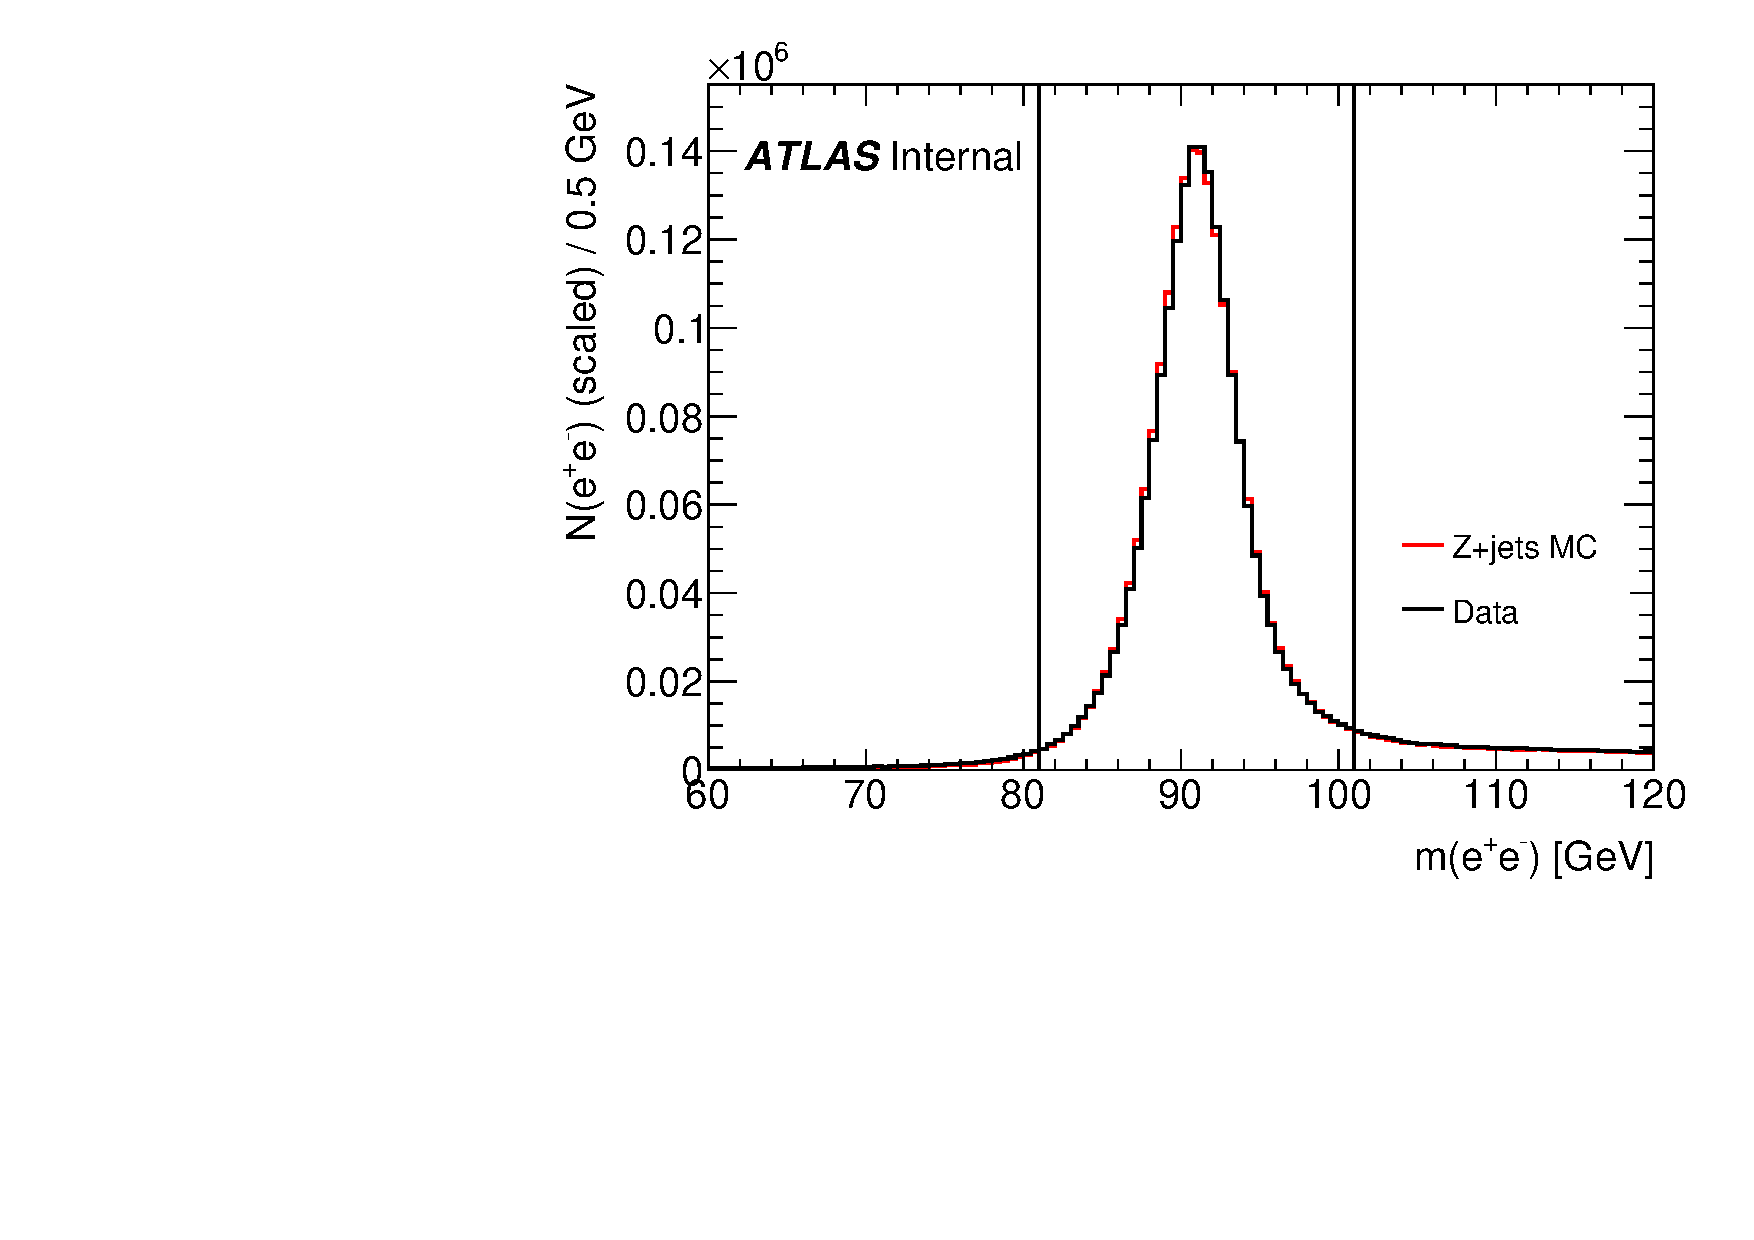
\includegraphics[width = 0.44 \textwidth]{figures/PhotonTrigEff/diph_mass.pdf}}
    \subfloat[]{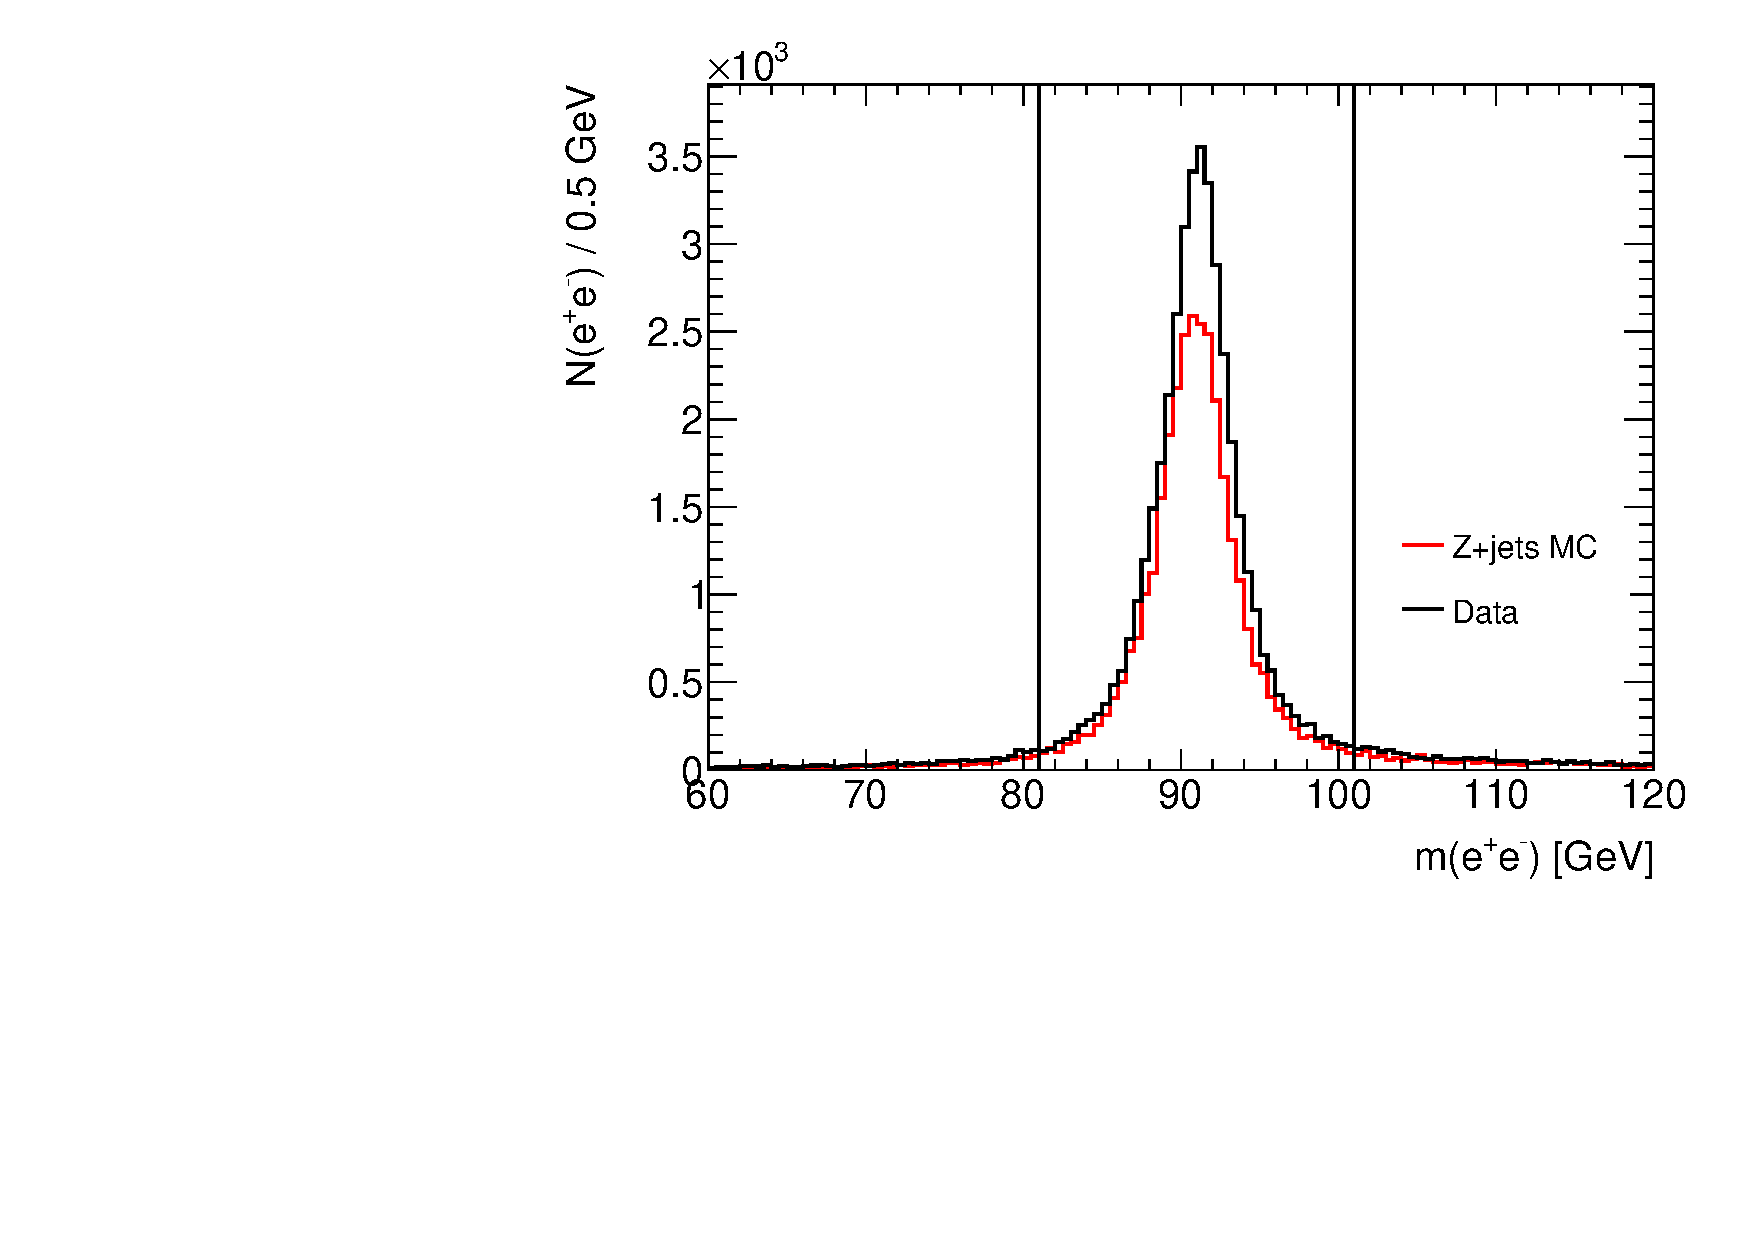
\includegraphics[width = 0.44 \textwidth]{figures/PhotonTrigEff/siph_mass.pdf}}
    \caption{Invariant mass distributions of the tag-and-probe electron pairs used to study the efficiencies of the (a) \texttt{HLT\_g50\_loose} and (b) \texttt{HLT\_g140\_loose} trigger in the data and $Z$+jets MC samples. Only the pairs with a probe electron in the plateau region of Figure~\ref{fig:PhotonTrigEff:di_pt} and~\ref{fig:PhotonTrigEff:si_pt} are considered.
    }
    \label{fig:PhotonTrigMass}
\end{figure}

The selected tag-and-probe electrons are used to estimate the efficiencies of photon triggers, shown as a function of probe $p_{T}$, $\eta$, and $|\zzero|$ in Figure~\ref{fig:PhotonTrigEff}. The efficiencies in $p_{T}$ show that the \texttt{HLT\_g50\_loose} plateau starts at $55 \si{\GeV}$, and \texttt{HLT\_g140\_loose} plateau starts at $148 \si{\GeV}$. The efficiencies in $\eta$ show good agreement between data and MC for electrons reconstructed inside the barrel, whereas small discrepancy in efficiencies are shown for electrons at the boundary regions and in the end-cap regions. Also, the efficiency in $|\zzero|$ shows no dependence of the photon trigger efficiencies on $|\zzero|$

\begin{figure}[!htb]
    \centering
    \subfloat[]{\label{fig:PhotonTrigEff:di_pt}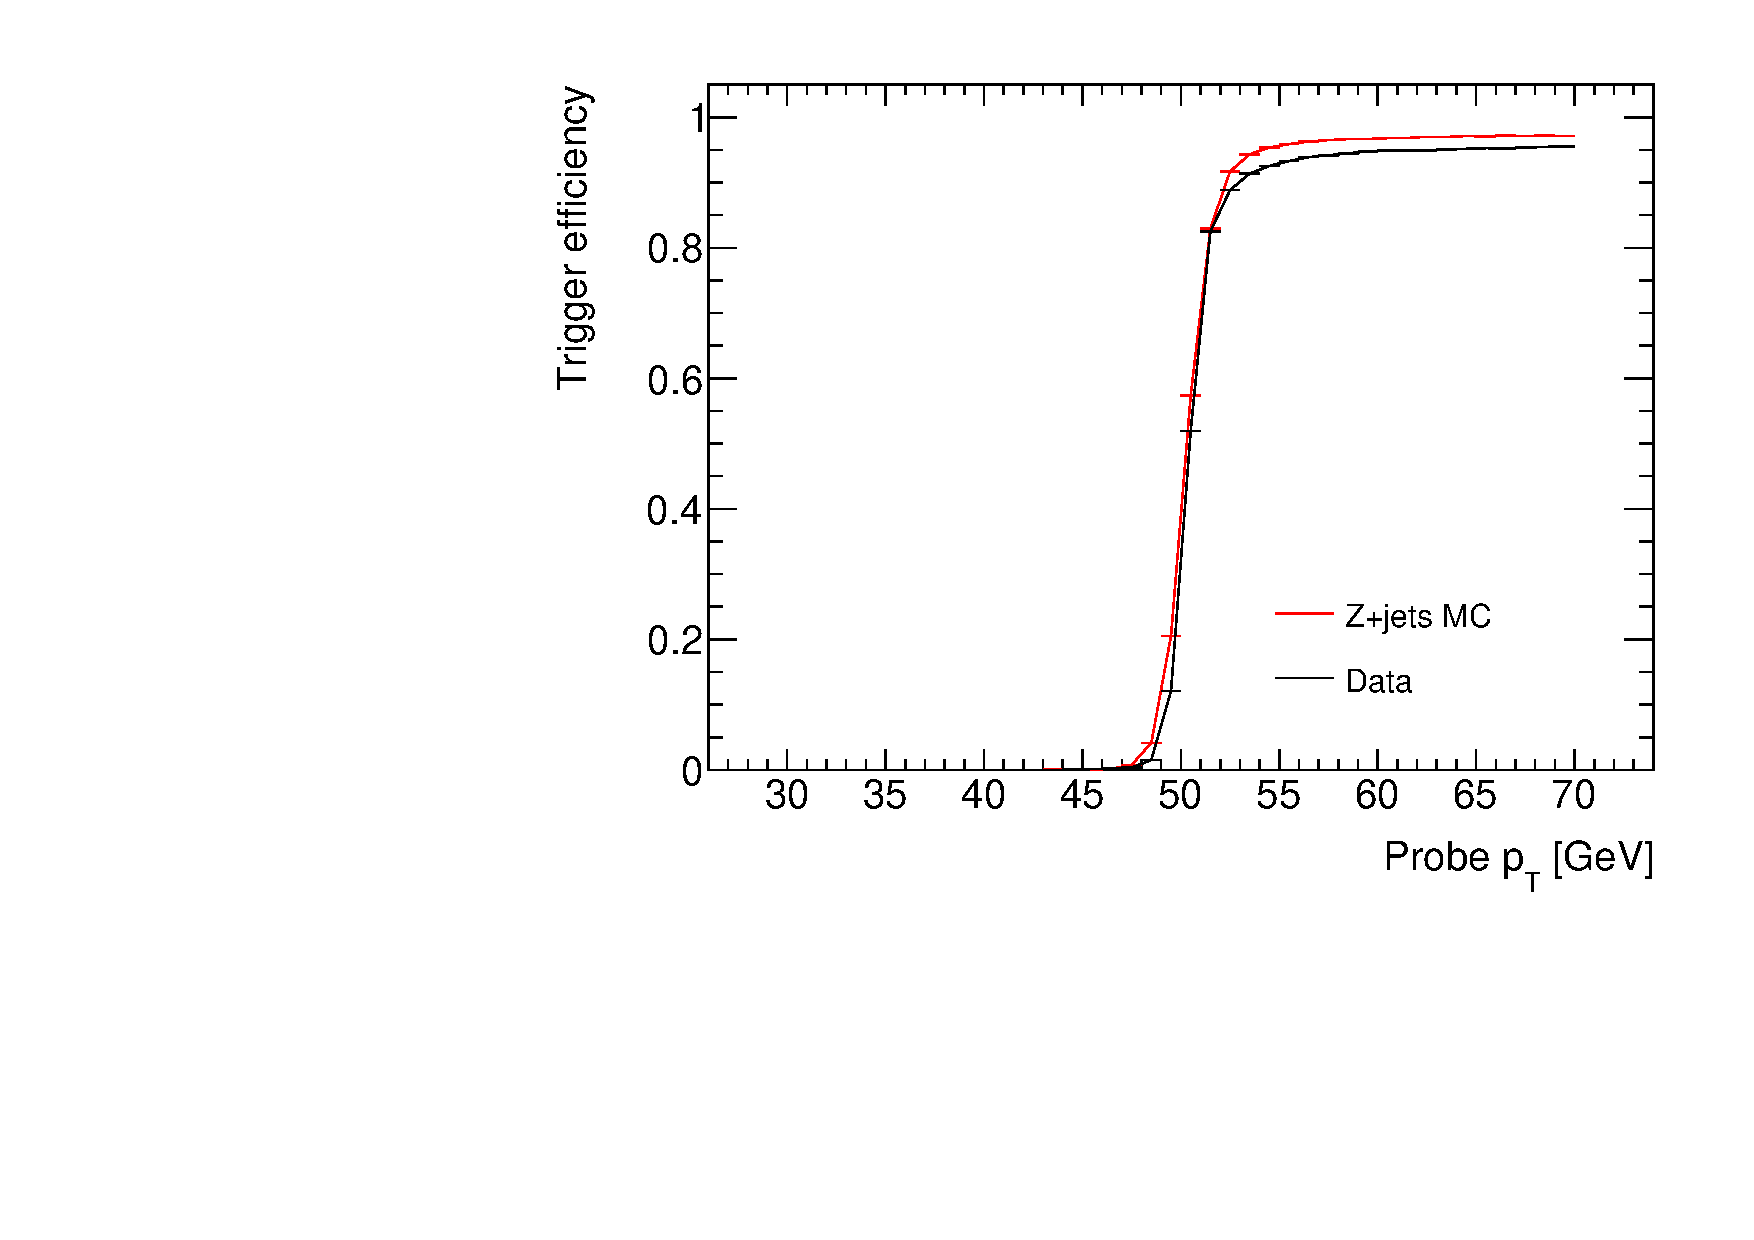
\includegraphics[width = 0.44 \textwidth]{figures/PhotonTrigEff/diph_eff_pt.pdf}}
    \subfloat[]{\label{fig:PhotonTrigEff:si_pt}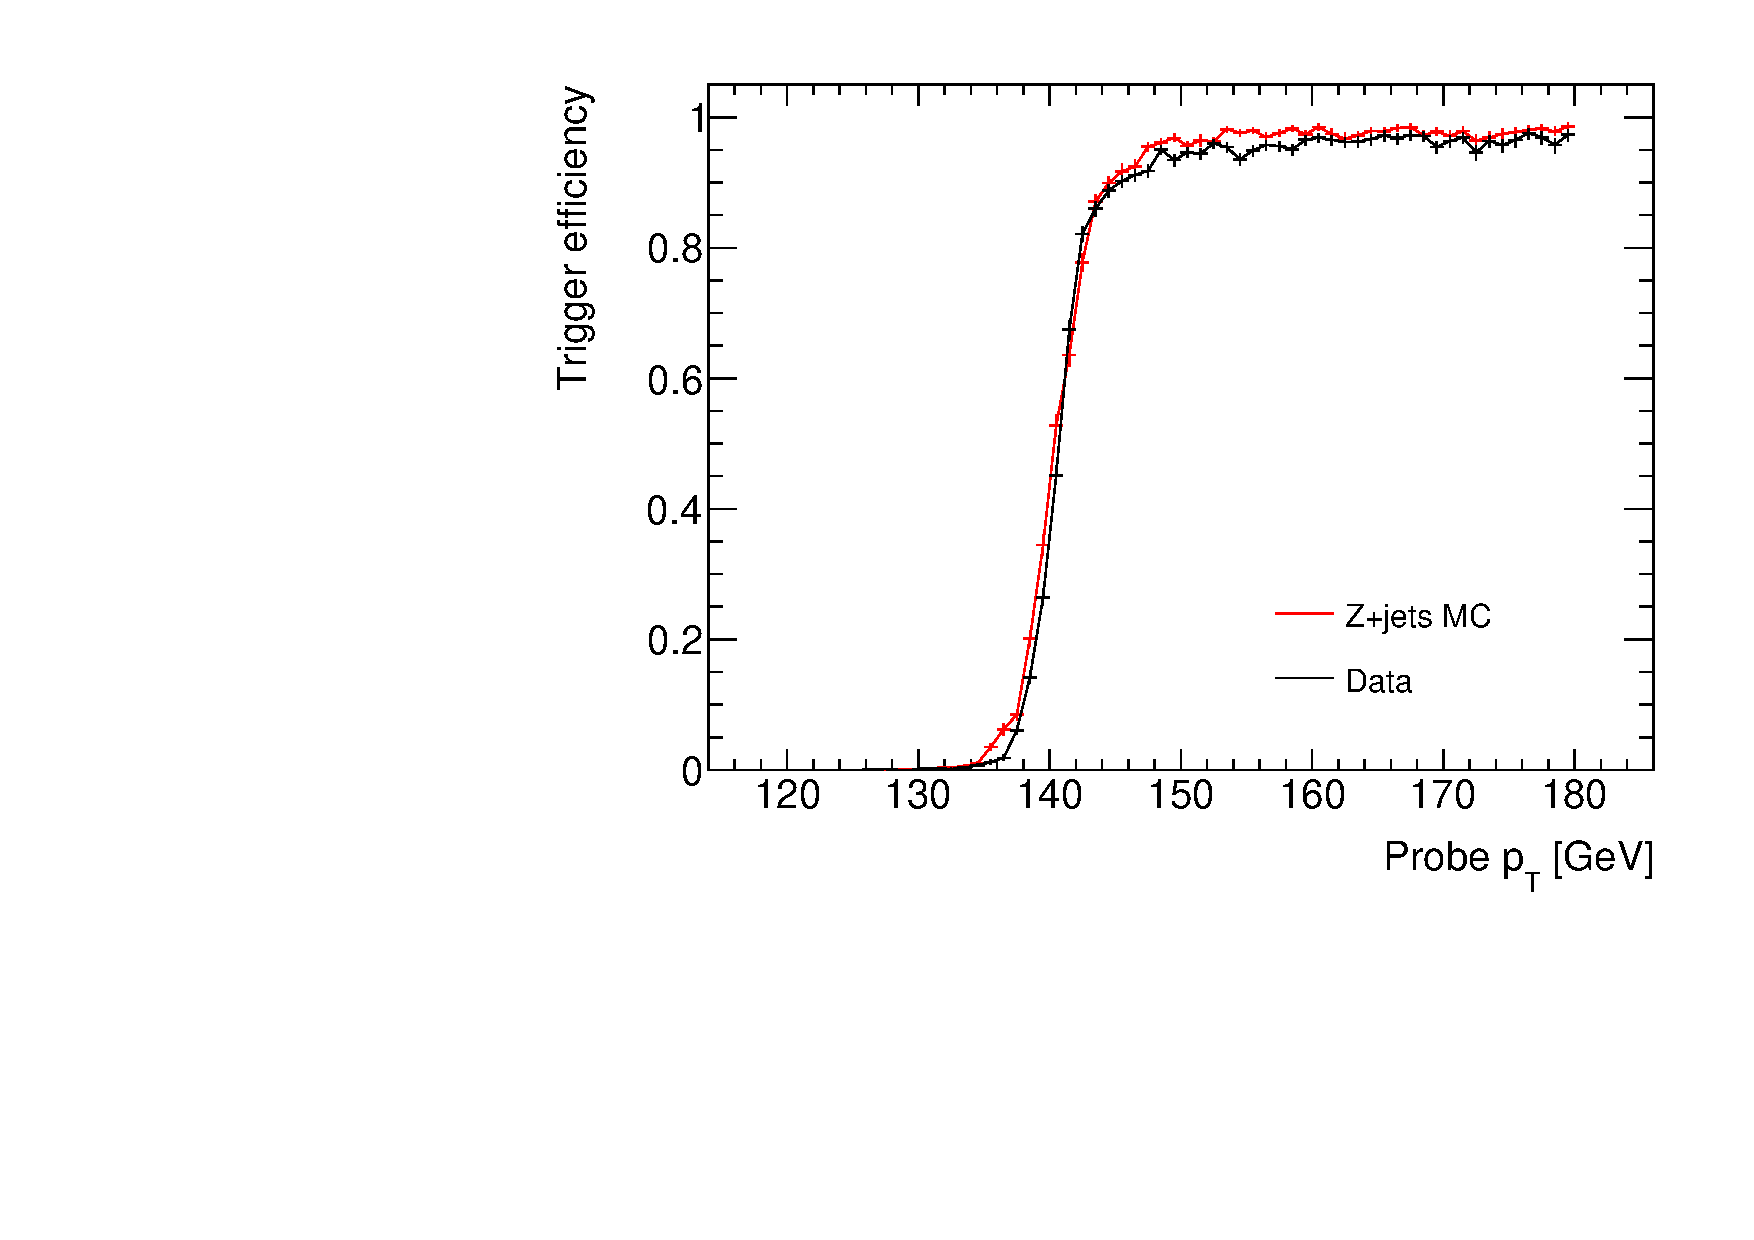
\includegraphics[width = 0.44 \textwidth]{figures/PhotonTrigEff/siph_eff_pt.pdf}} \\
    \subfloat[]{\label{fig:PhotonTrigEff:di_eta}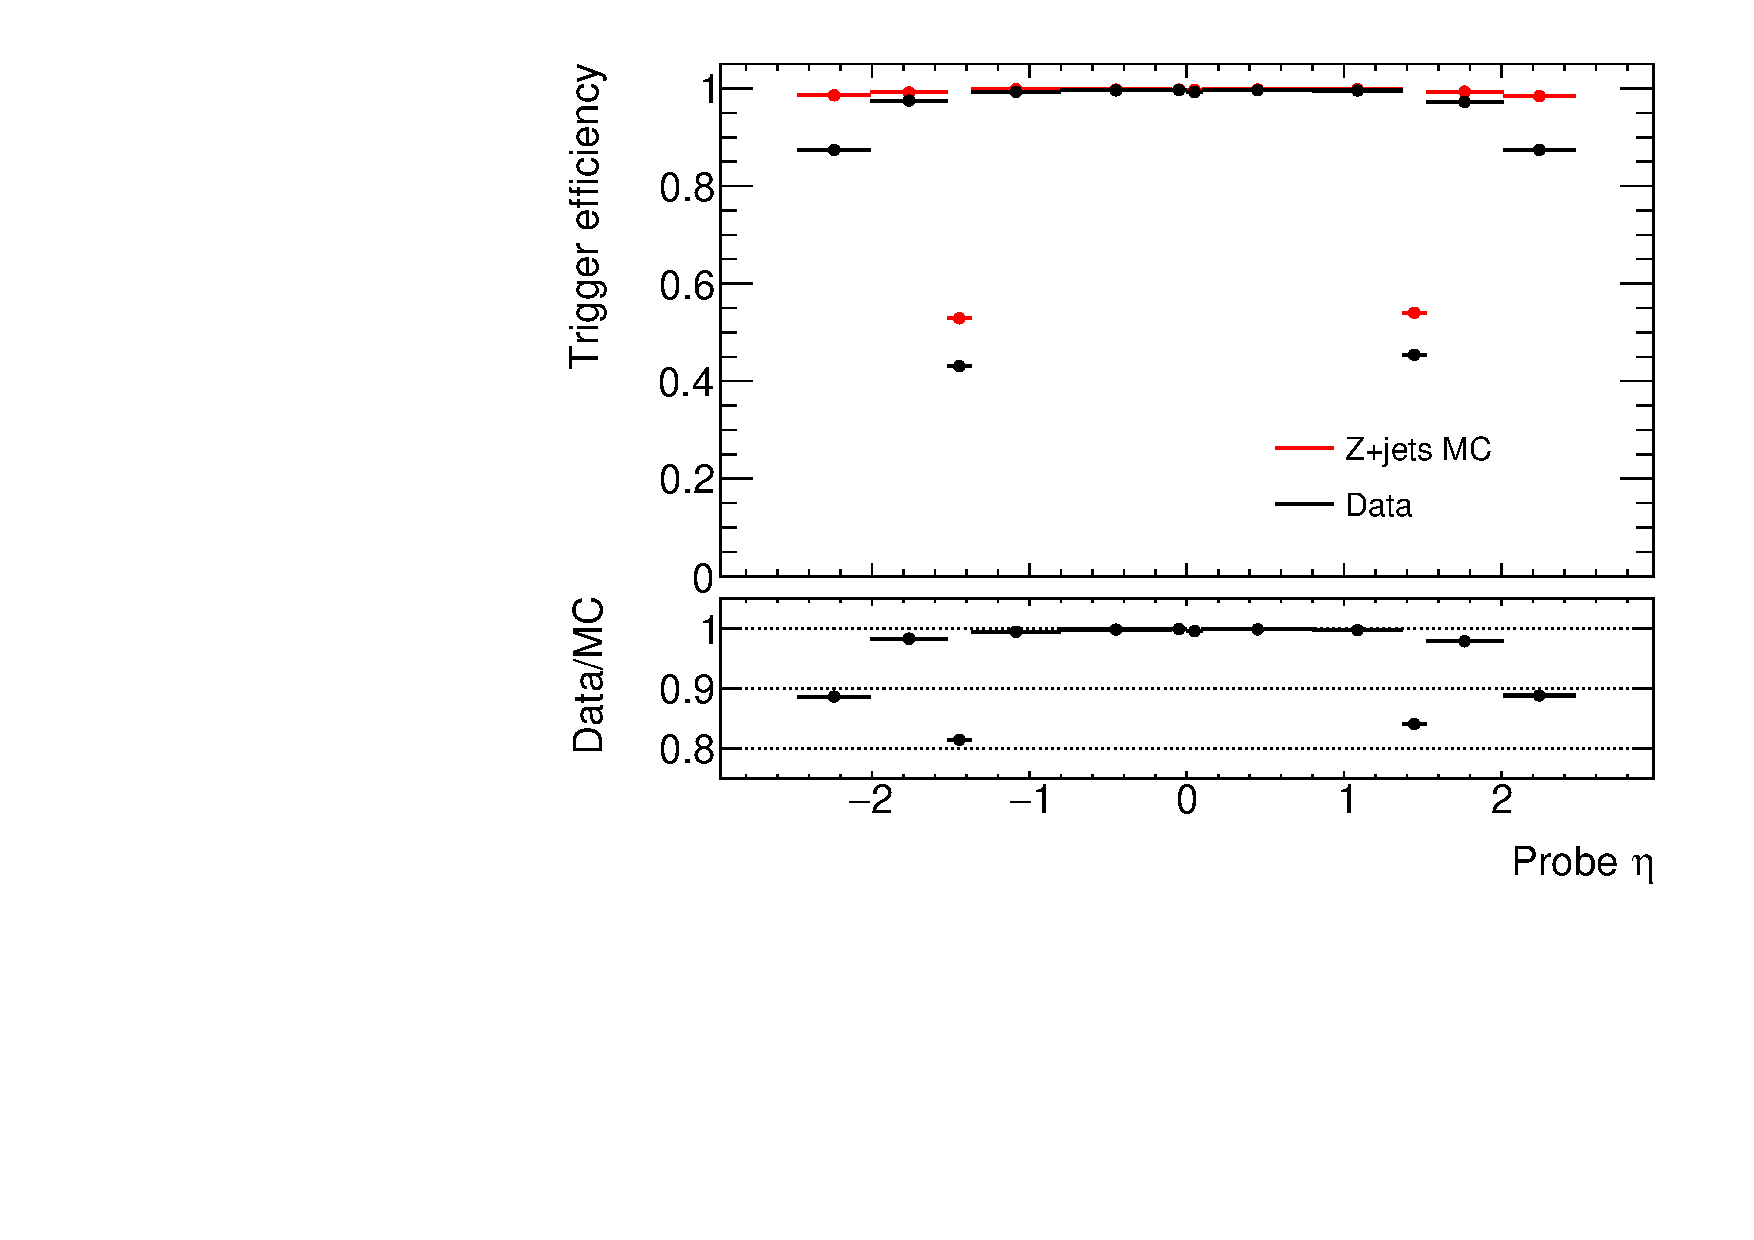
\includegraphics[width = 0.44 \textwidth]{figures/PhotonTrigEff/diph_eff_eta.pdf}}
    \subfloat[]{\label{fig:PhotonTrigEff:si_eta}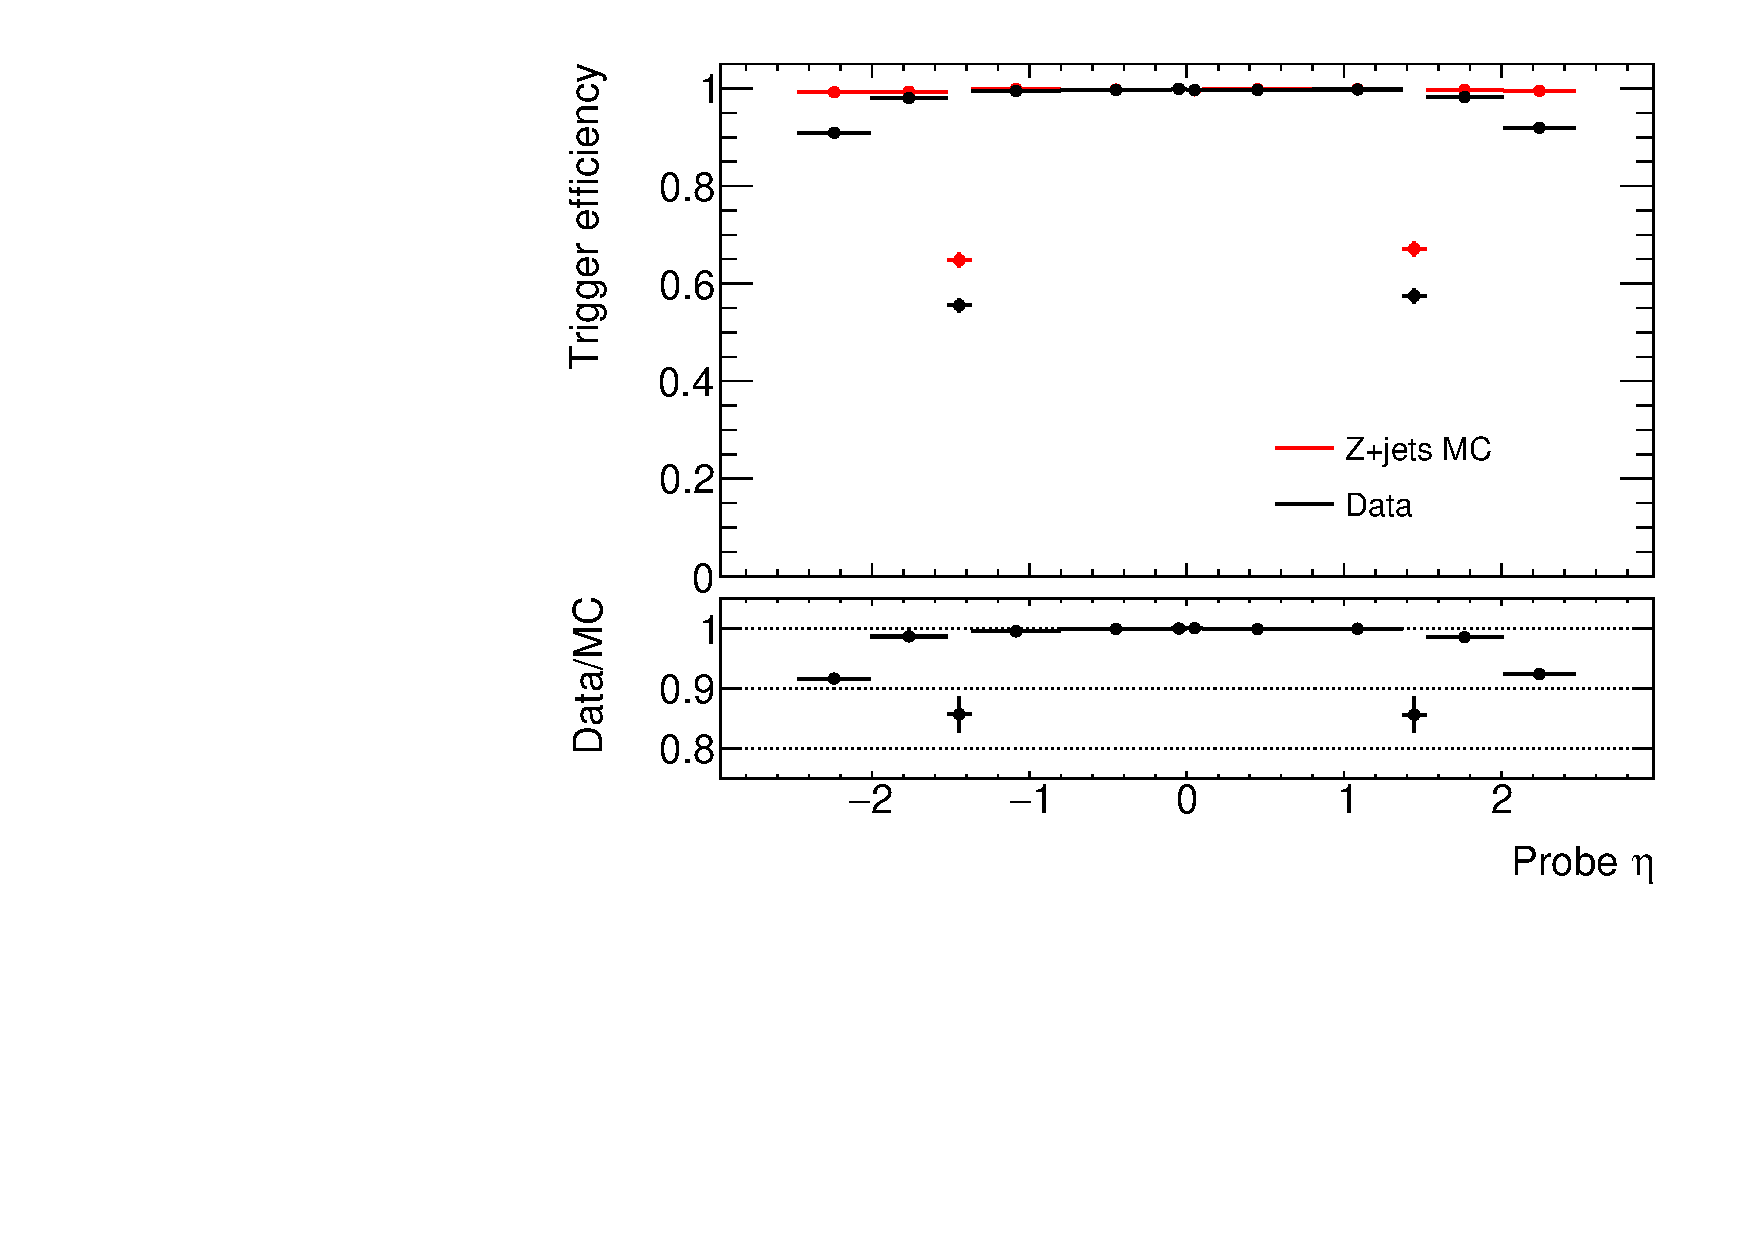
\includegraphics[width = 0.44 \textwidth]{figures/PhotonTrigEff/siph_eff_eta.pdf}} \\
    \subfloat[]{\label{fig:PhotonTrigEff:di_z0}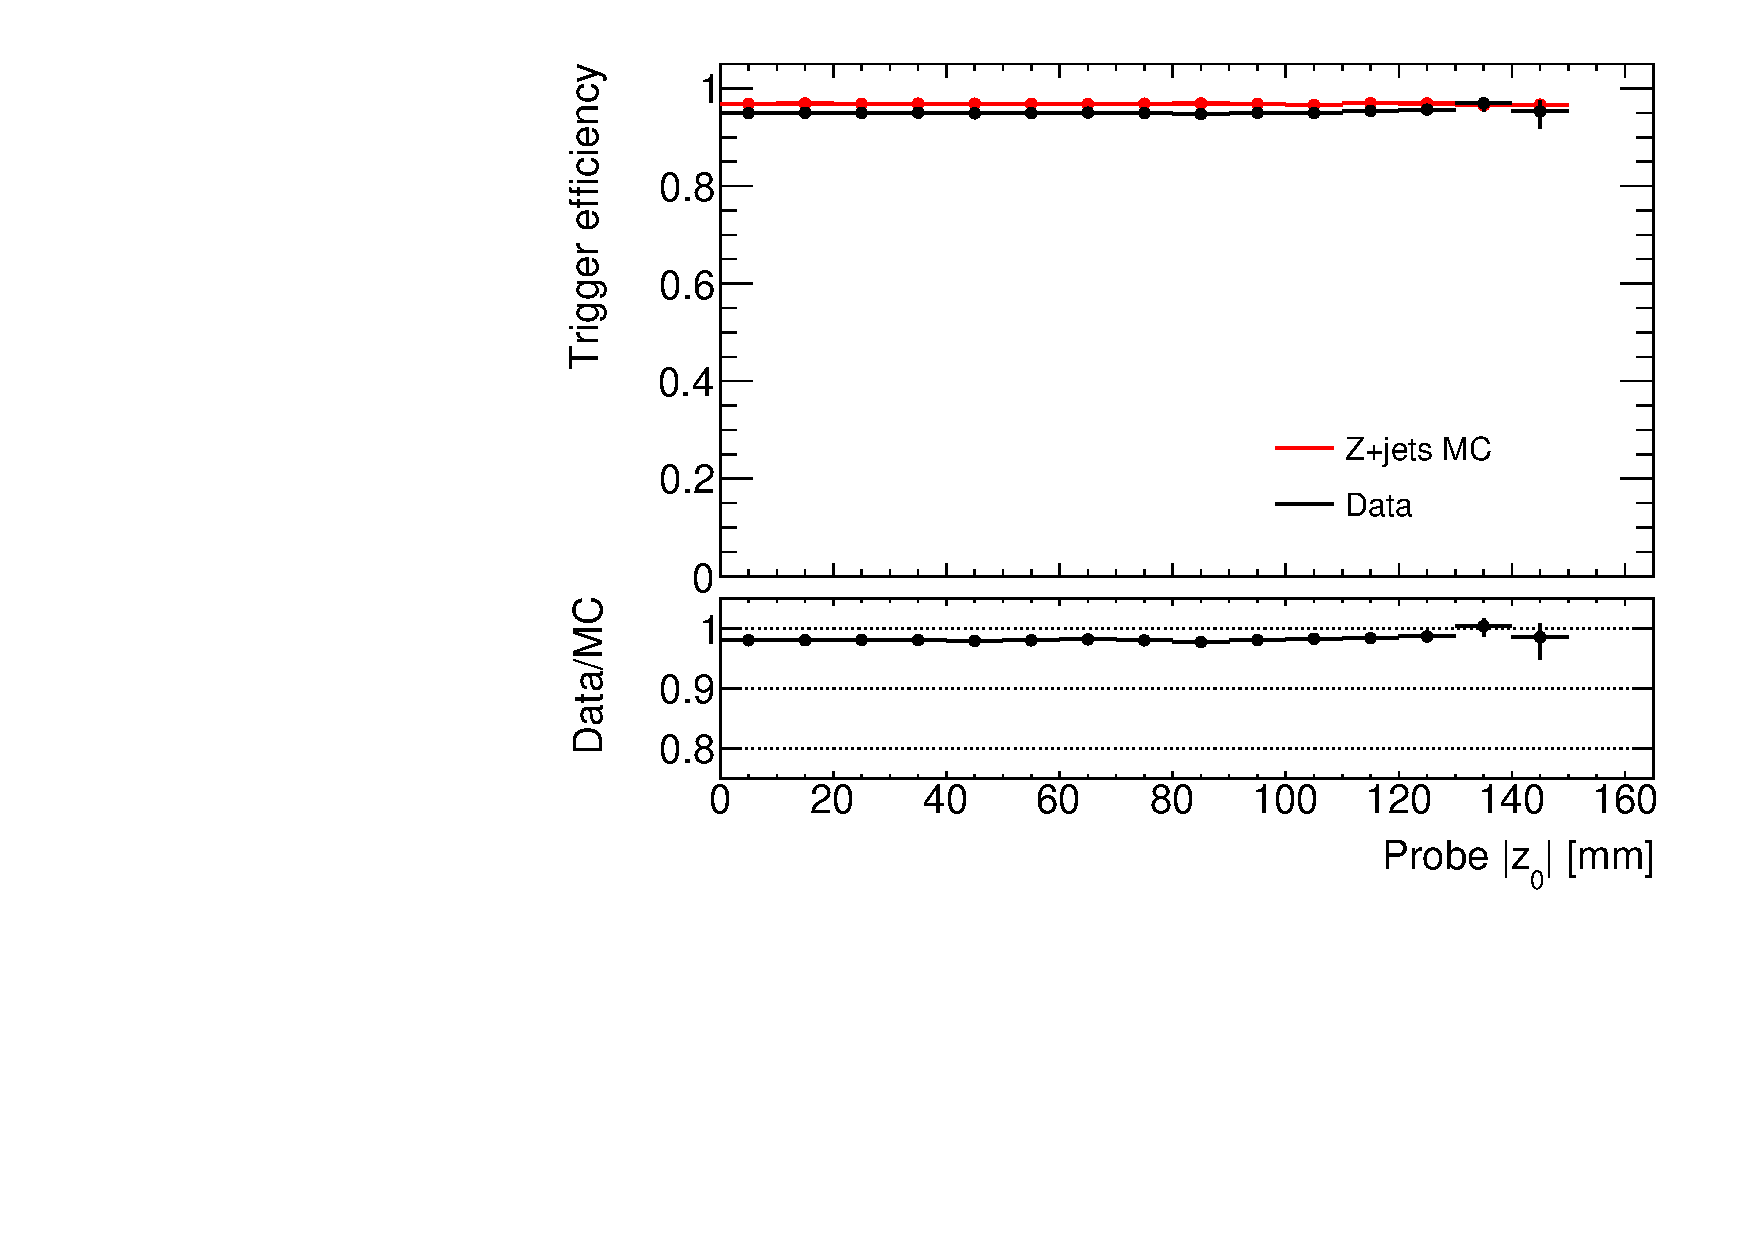
\includegraphics[width = 0.44 \textwidth]{figures/PhotonTrigEff/diph_eff_z0.pdf}}
    \subfloat[]{\label{fig:PhotonTrigEff:si_z0}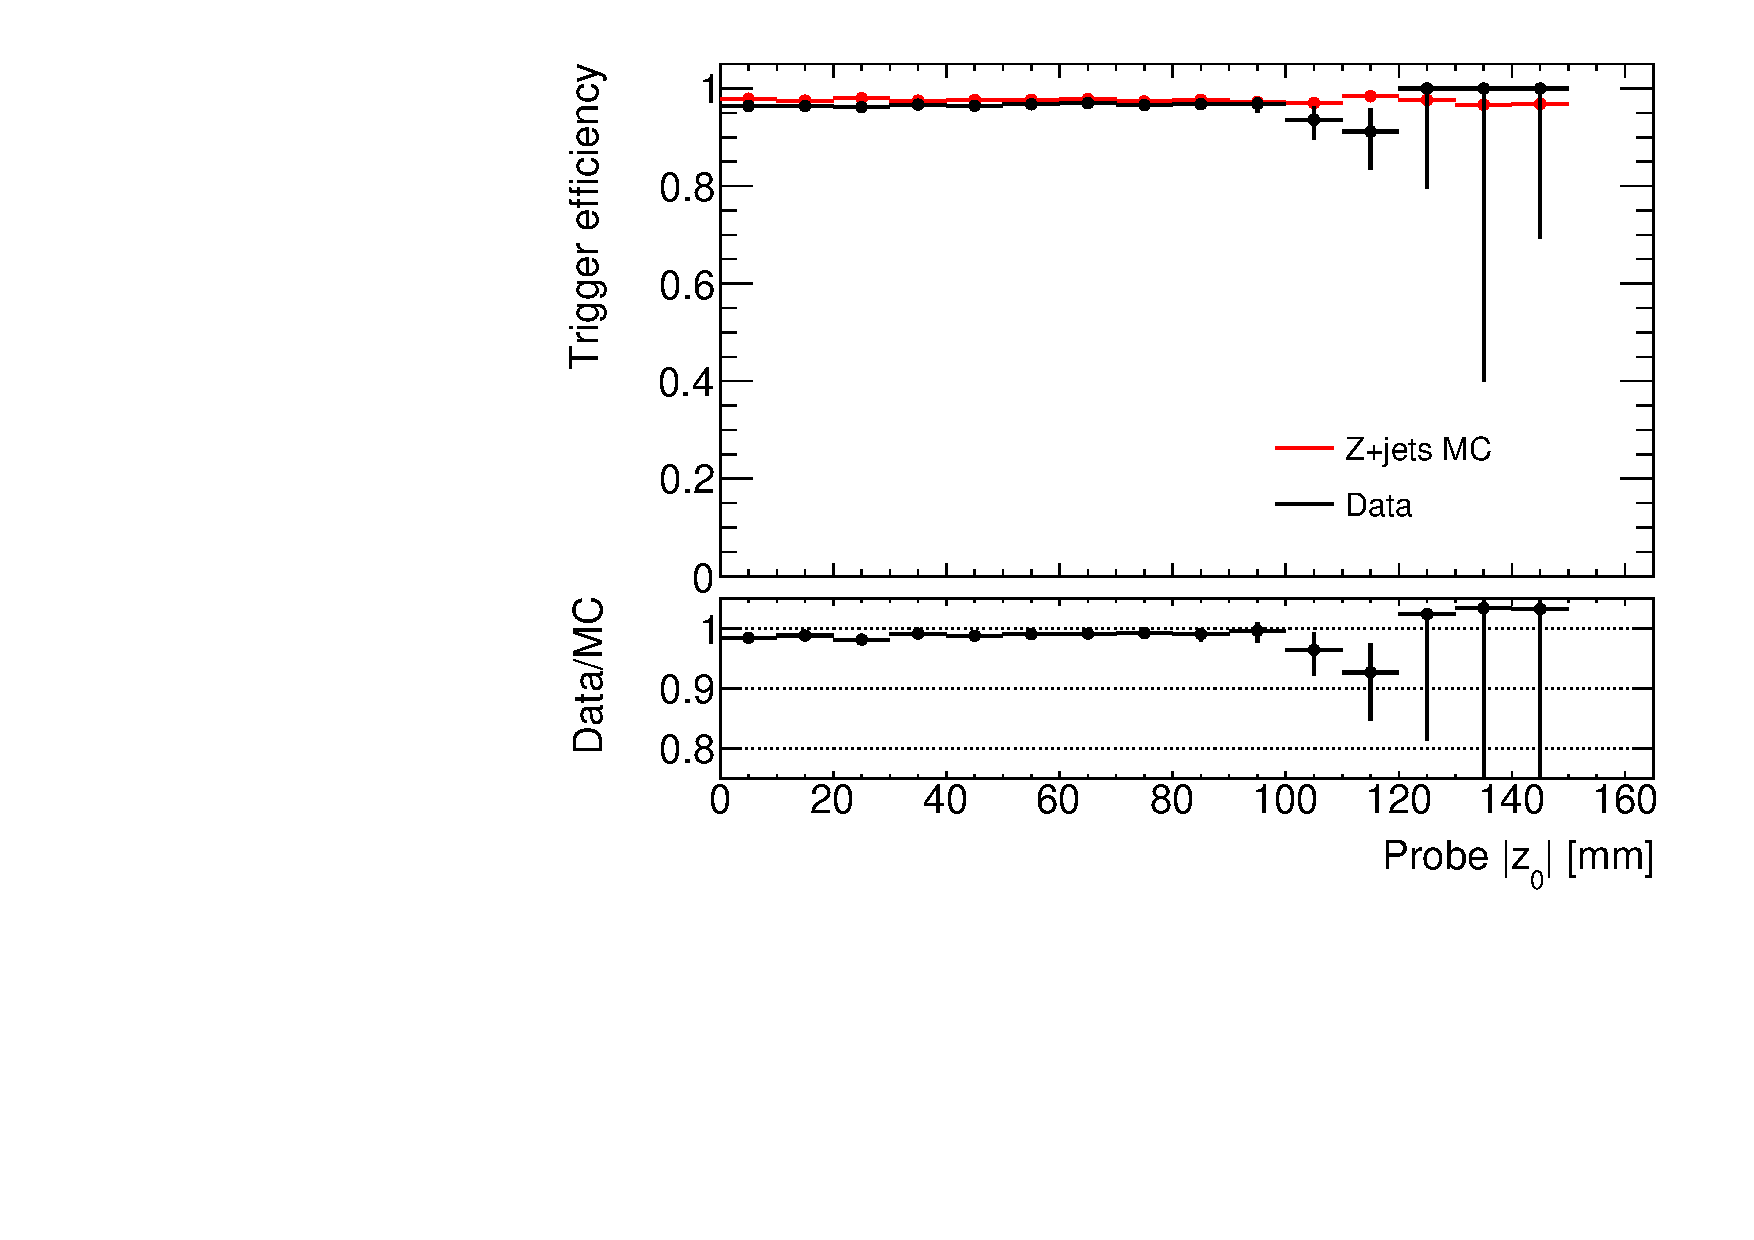
\includegraphics[width = 0.44 \textwidth]{figures/PhotonTrigEff/siph_eff_z0.pdf}}
    \caption{Efficiencies of the \texttt{HLT\_g50\_loose} as a function of probe (a) $p_{T}$, (c) $\eta$, and (e) $|\zzero|$ estimated using the data and $Z$+jets MC samples. The corresponding plots of the \texttt{HLT\_g140\_loose} trigger are shown in (b), (d), and (f). Only the pairs with a probe electron in the plateau region of (a) and (b) are considered in the rest.
    }
    \label{fig:PhotonTrigEff}
\end{figure}




\subsection{Muon trigger}
\label{subsect:muonTrigEff}

The systematic uncertainty of the single muon trigger is estimated with a standard tag-and-probe method on $Z \rightarrow \mu\mu$ events both in data and MC. The selection criteria of muon tag-and-probe candidates are listed in Table~\ref{tab:ZmmSelection}. Similar to the photon triggers, pairs are required to have opposite signs and to satisfy the mass requirement ($|m_{e^{+}e^{-}} - m_{Z}| < 10~\si{\GeV}$) and the isolation requirement of $\DeltaR(\mathrm{tag}, \mathrm{probe}) > 0.4$. 

\begin{table}[!htb]
	\centering
	\begin{tabular}{ccc}
		\hline
		\hline
		Cut & Tag muon & Probe muon \\
		\hline
		$p_{T}$ [GeV] $>$ & 28 & 30 \\
		Trigger matched & \texttt{HLT\_mu26\_ivarmedium} & --- \\
		$|\eta| <$ & 2.4 & 1.05 \\
		Identification & Medium & Loose and combined \\
		Isolation & Loose & --- \\
		\dzero significance & $< 3$ & --- \\
		$\Delta \zzero \sin{\theta}$ & $< 0.5 \si{\mm}$ & --- \\
		\hline
		\hline
	\end{tabular}
	\caption{Selection criteria for tag-and-probe muons.}
	\label{tab:ZmmSelection}
\end{table}

The invariant mass distributions of the muon tag-and-probe pairs found in the data and the MC samples are shown in Figure~\ref{fig:MuonTrigMass}. The shape of distribution is in good agreement with negligible background. Therefore, no background subtraction is performed in the calculation of the trigger efficiency.

\begin{figure}[!htb]
    \centering
    \subfloat{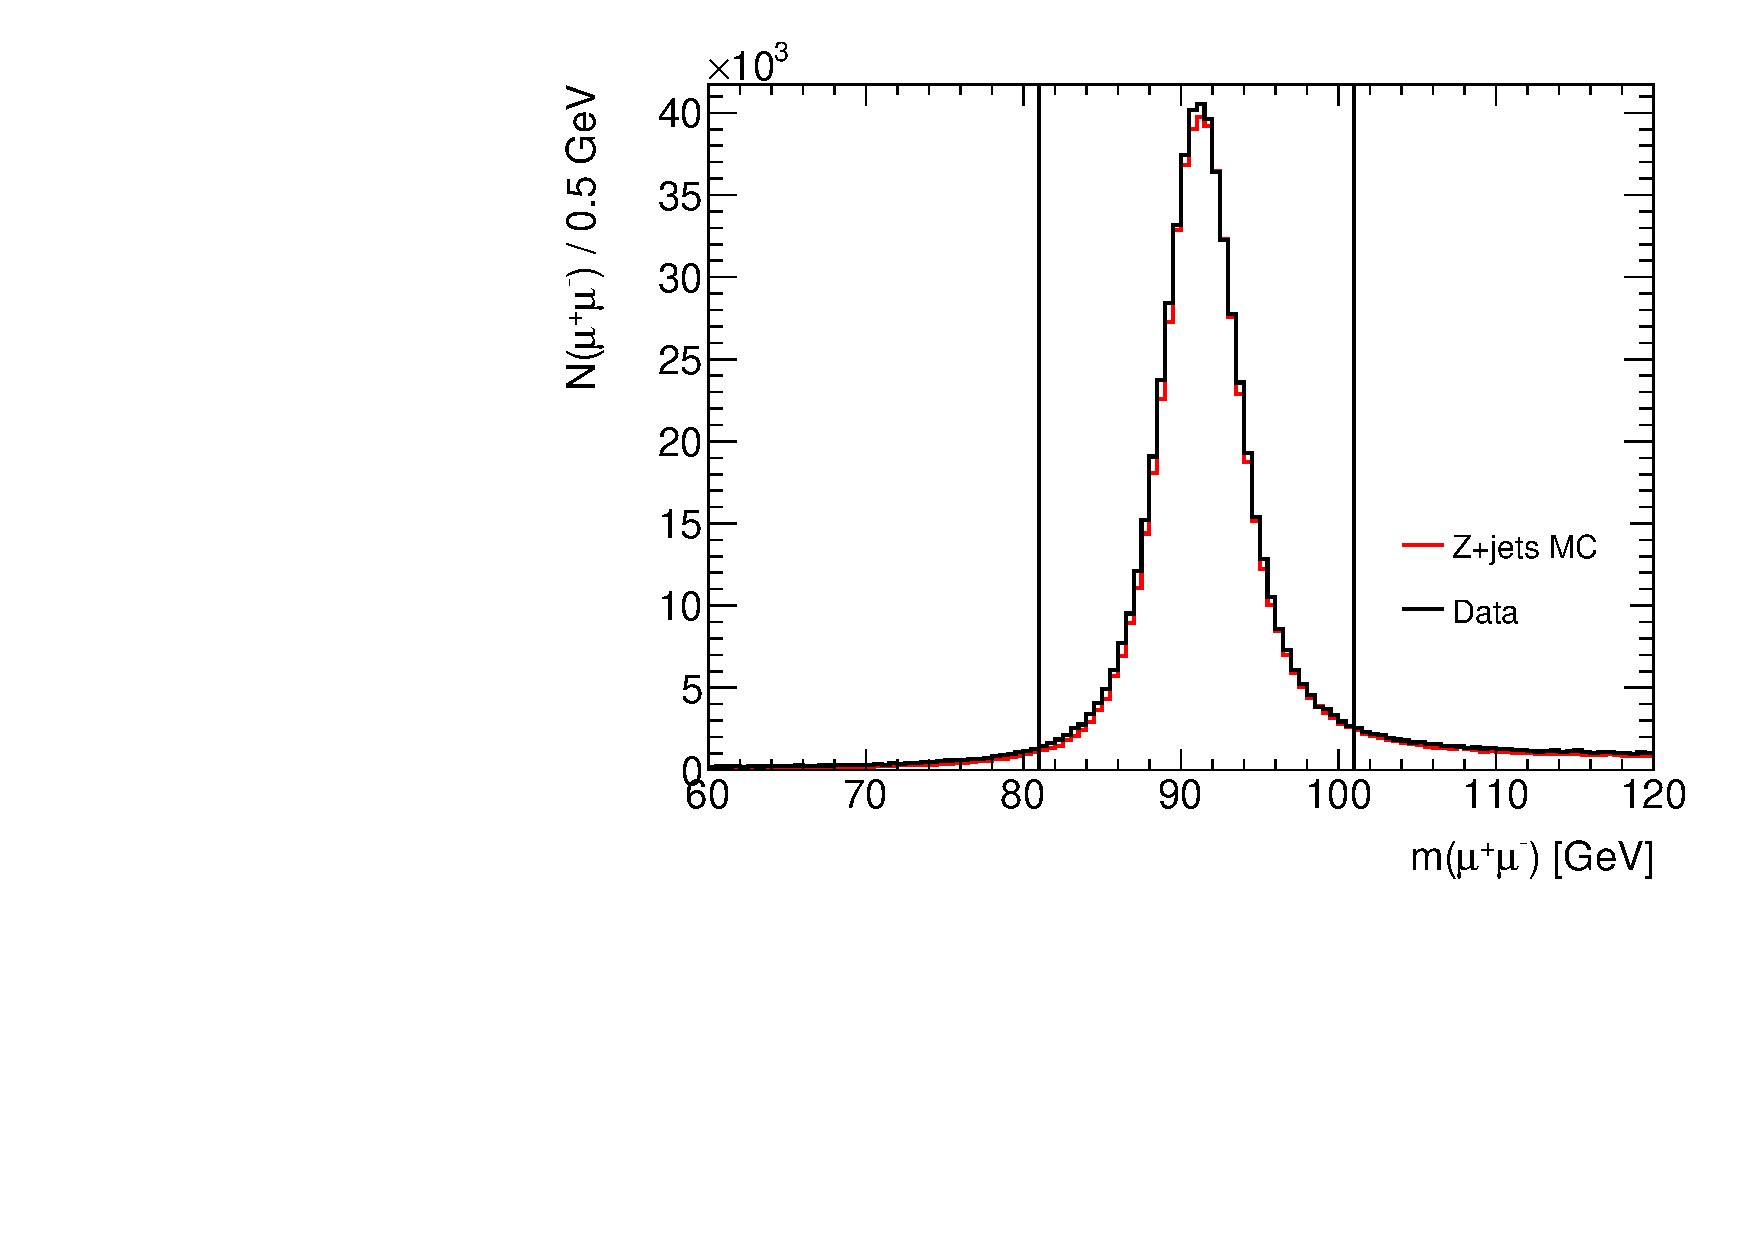
\includegraphics[width = 0.44 \textwidth]{figures/MuonTrigEff/mass.pdf}}
    \caption{Invariant mass distributions of the tag-and-probe muon pairs used to study the efficiencies of the single muon trigger in the data and $Z$+jets MC samples. Only the pairs with a probe muon in the plateau region of Figure~\ref{fig:MuonTrigEff1Da} are considered.
    }
    \label{fig:MuonTrigMass}
\end{figure}

The selected tag-and-probe muons are used to estimate the efficiency of the single muon trigger, shown as a function of probe $p_{T}$ and $|\zzero|$ in Figure~\ref{fig:MuonTrigEff1D}. The efficiency in $p_{T}$ show that the muon trigger plateau starts at $62 \si{\GeV}$. The efficiency in $|\zzero|$ shows no dependence of the muon trigger efficiency on $|\zzero|$. However, the trigger efficiency in data can be studied up to $|\zzero| \sim150~\si{\mm}$ at which a significant decrease in the efficiency is shown.


\begin{figure}[!htb]
    \centering
    \subfloat[\label{fig:MuonTrigEff1Da}]{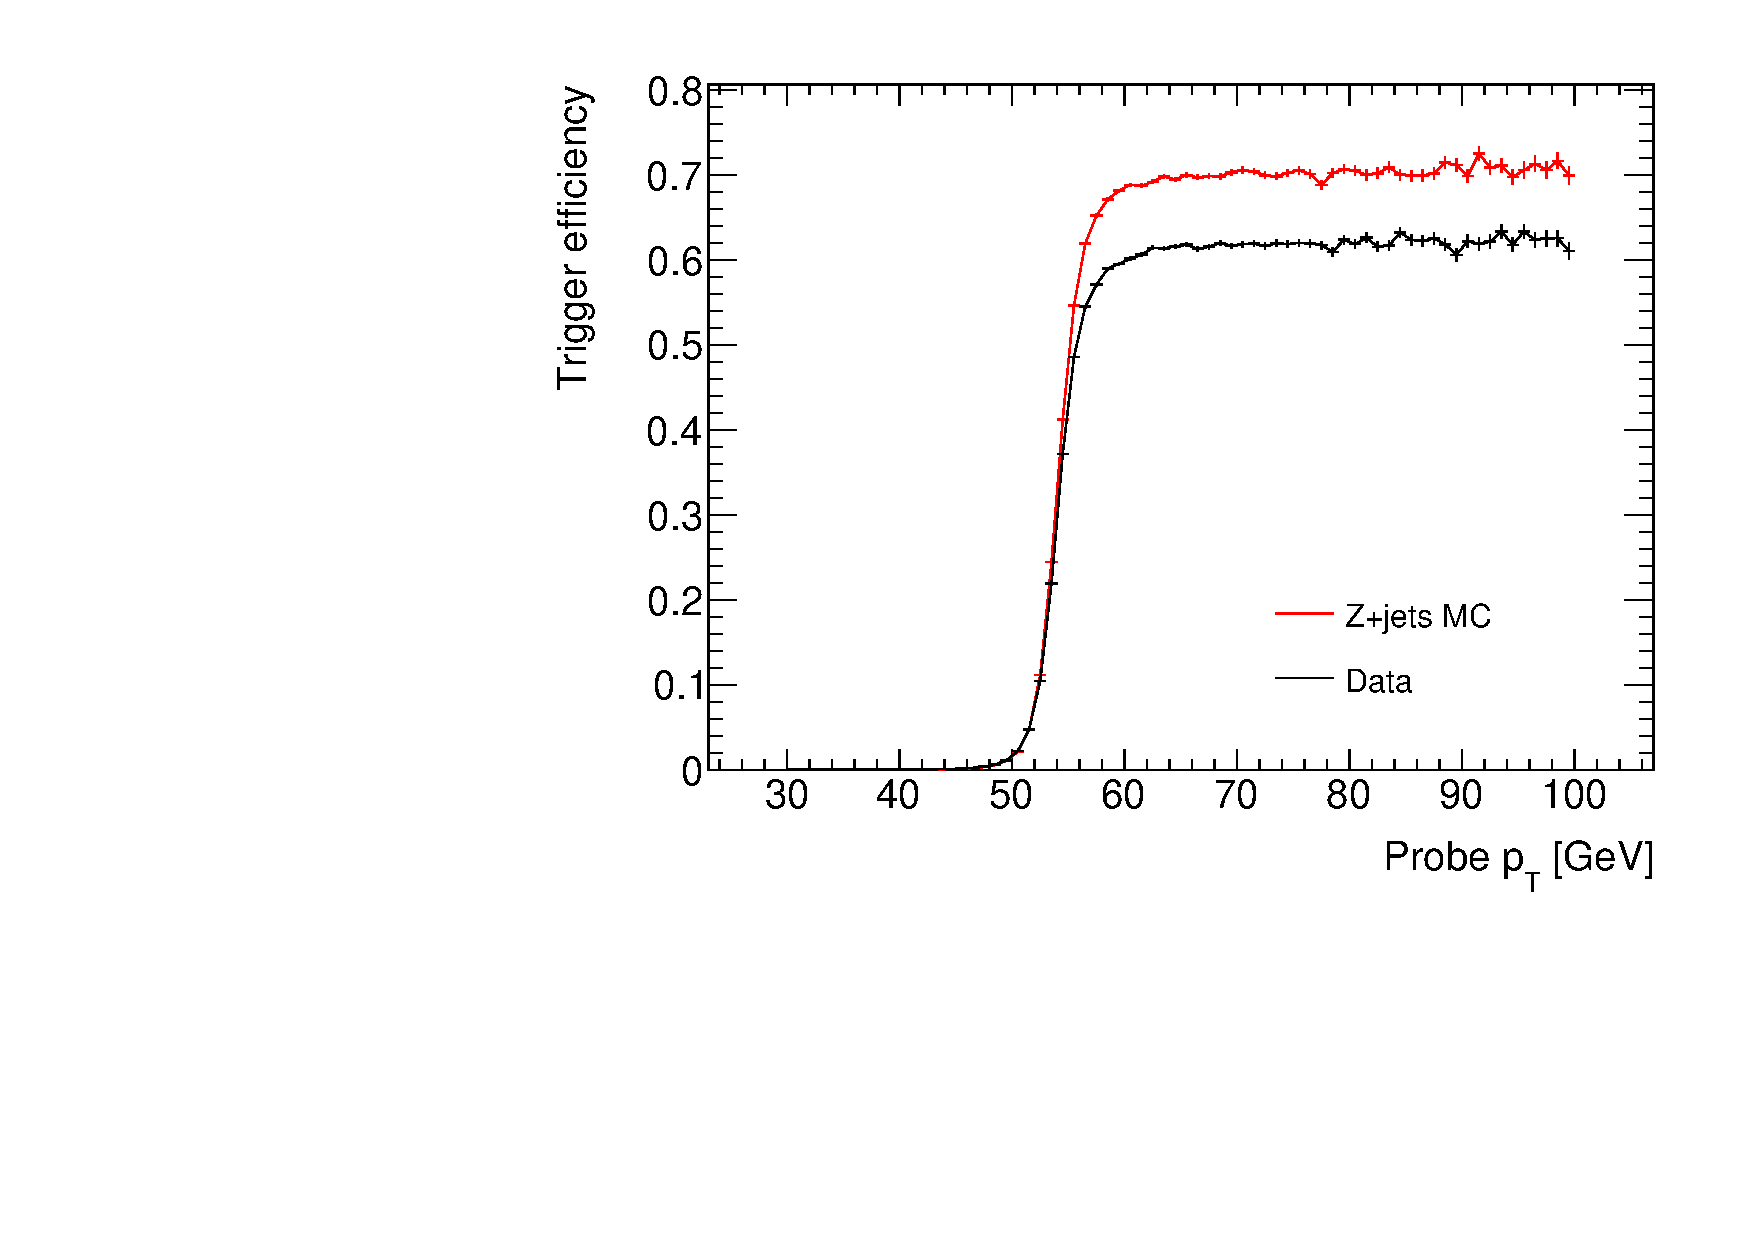
\includegraphics[width = 0.44 \textwidth]{figures/MuonTrigEff/simu_pt.pdf}}
    \subfloat[\label{fig:MuonTrigEff1Db}]{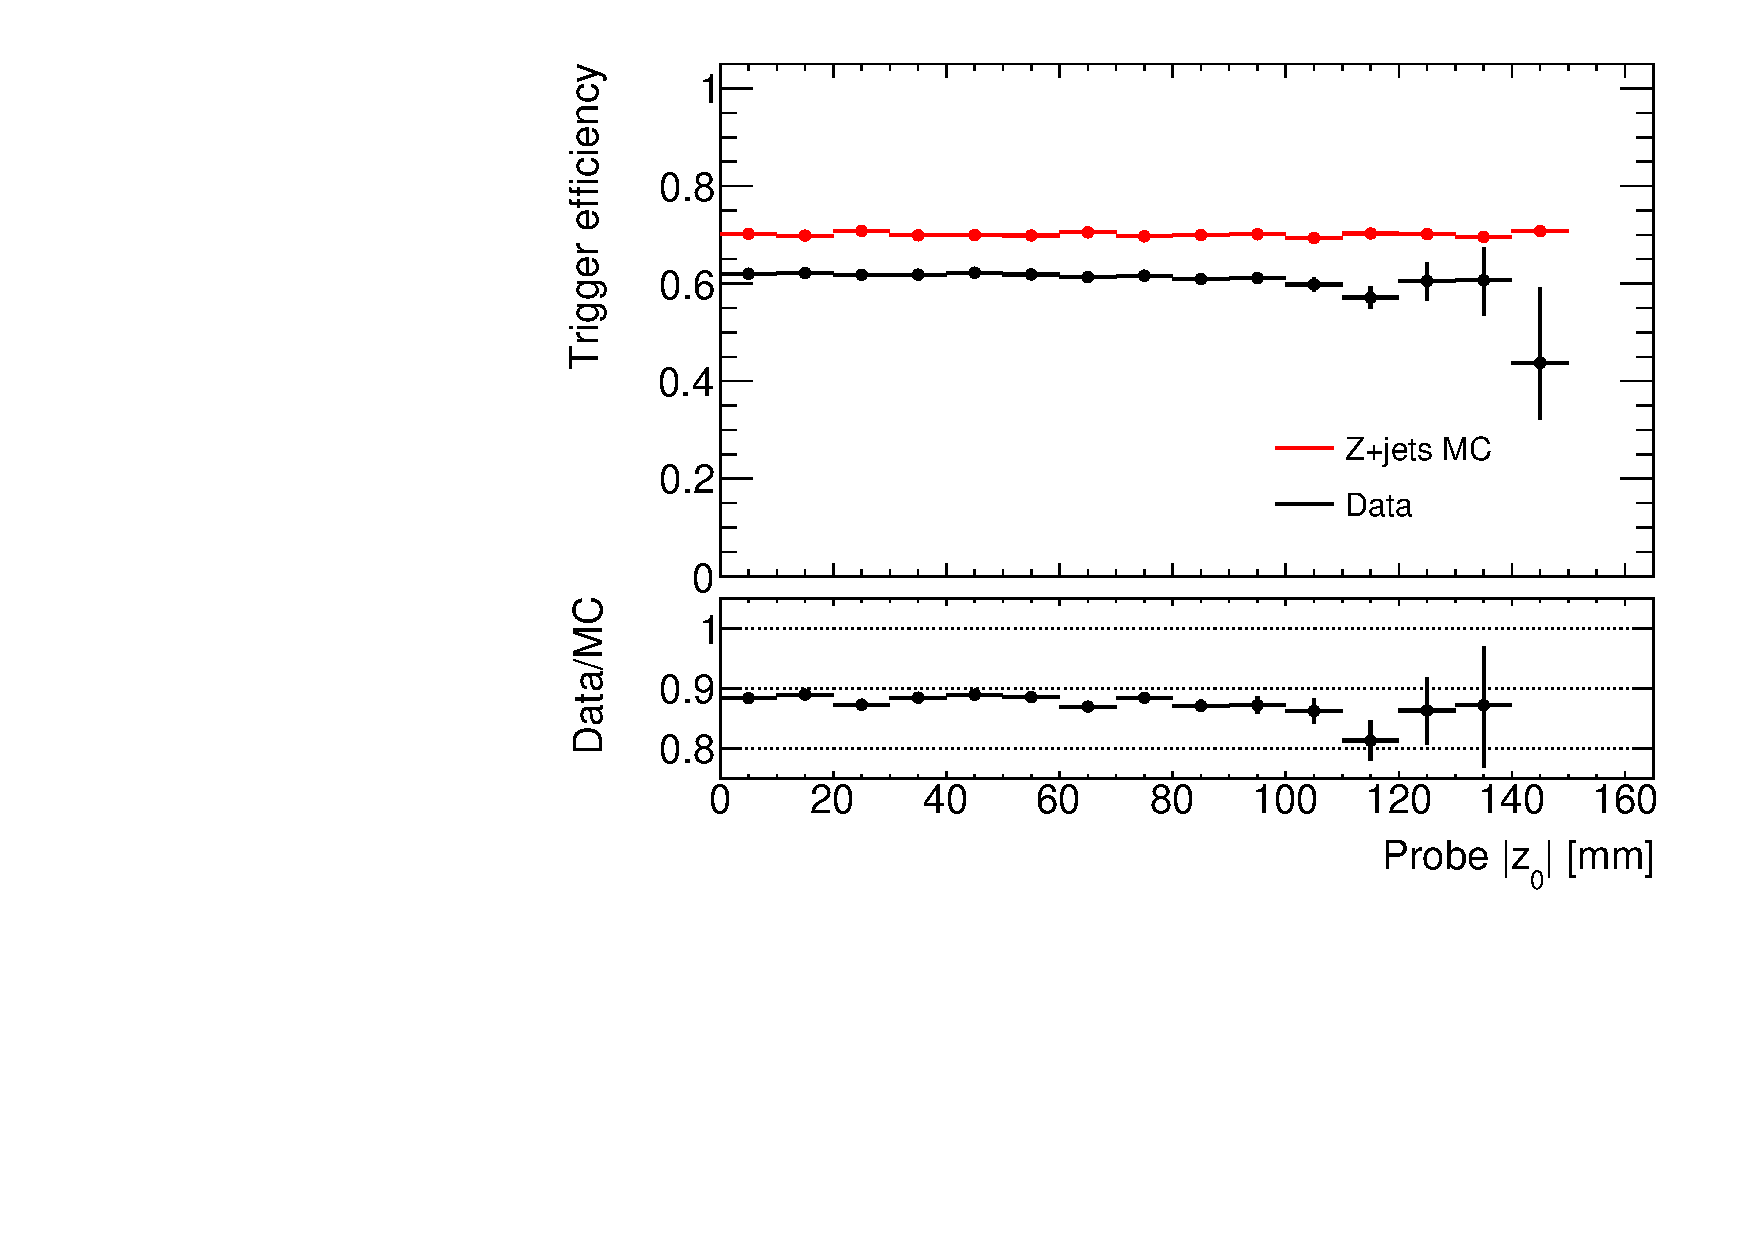
\includegraphics[width = 0.44 \textwidth]{figures/MuonTrigEff/simu_z0.pdf}}
    \caption{Efficiency of the single muon trigger as a function of probe (a) $p_{T}$ and (b) |\zzero| estimated using the data and $Z$+jets MC samples. Only the pairs with a probe electron in the plateau region of (a) are considered in (b).}
    \label{fig:MuonTrigEff1D}
\end{figure}





\begin{table}[!htb]
	\centering
	\begin{tabular}{cc}
		\hline
		\hline
		Source                              &       Syst. Uncert.       \\
		\hline
        Trigger                             &       -                   \\
        Track and vertex reconstruction     &       40\%                \\
		\hline
        Total                               &       15\%                \\
		\hline
		\hline
	\end{tabular}
	\caption{Summary table of all systematic uncertainties in the signal efficiency}
	\label{tab:syst_total}
\end{table}


























